\chapter{Studies with the Soft Muon Tagger}
Analyses that involve final states with $b$-quarks heavily rely on the accurate identification of these quarks. Ongoing efforts are dedicated to refine this identification process. This chapter presents a study on how muons can contribute to the identification of $b$-quarks in current $b$-tagging algorithms applied to small-$R$ jets.


\section{Soft Muon tagging}
\label{sec:SoftMuonTagging}
Algorithms currently in use for $b$-tagging described in section \ref{sec:b_tagging}, primarily exploit the displaced secondary vertex that is characteristic of the long lifetime of $b$-quarks. Besides vertex finding algorithms muons can be used as indication for the presence of a $b$-hadron.This is because approximately \qty{20}{\percent} of the $b$-jets undergo semi-leptonic decays that involve a muon as exemplified in figure \ref{fig:semileptonicDecay}. The branching fractions for these decays are roughly \qty{11}{\percent} for direct $b$ to muon decays $BR( b \rightarrow \mu \nu X )$ and about \qty{10}{\percent} for cascade decays $BR( b \rightarrow c \rightarrow \mu \nu X )$ \citep{expectedPerformanceAtlas}.
\begin{figure}[]
  \centering
  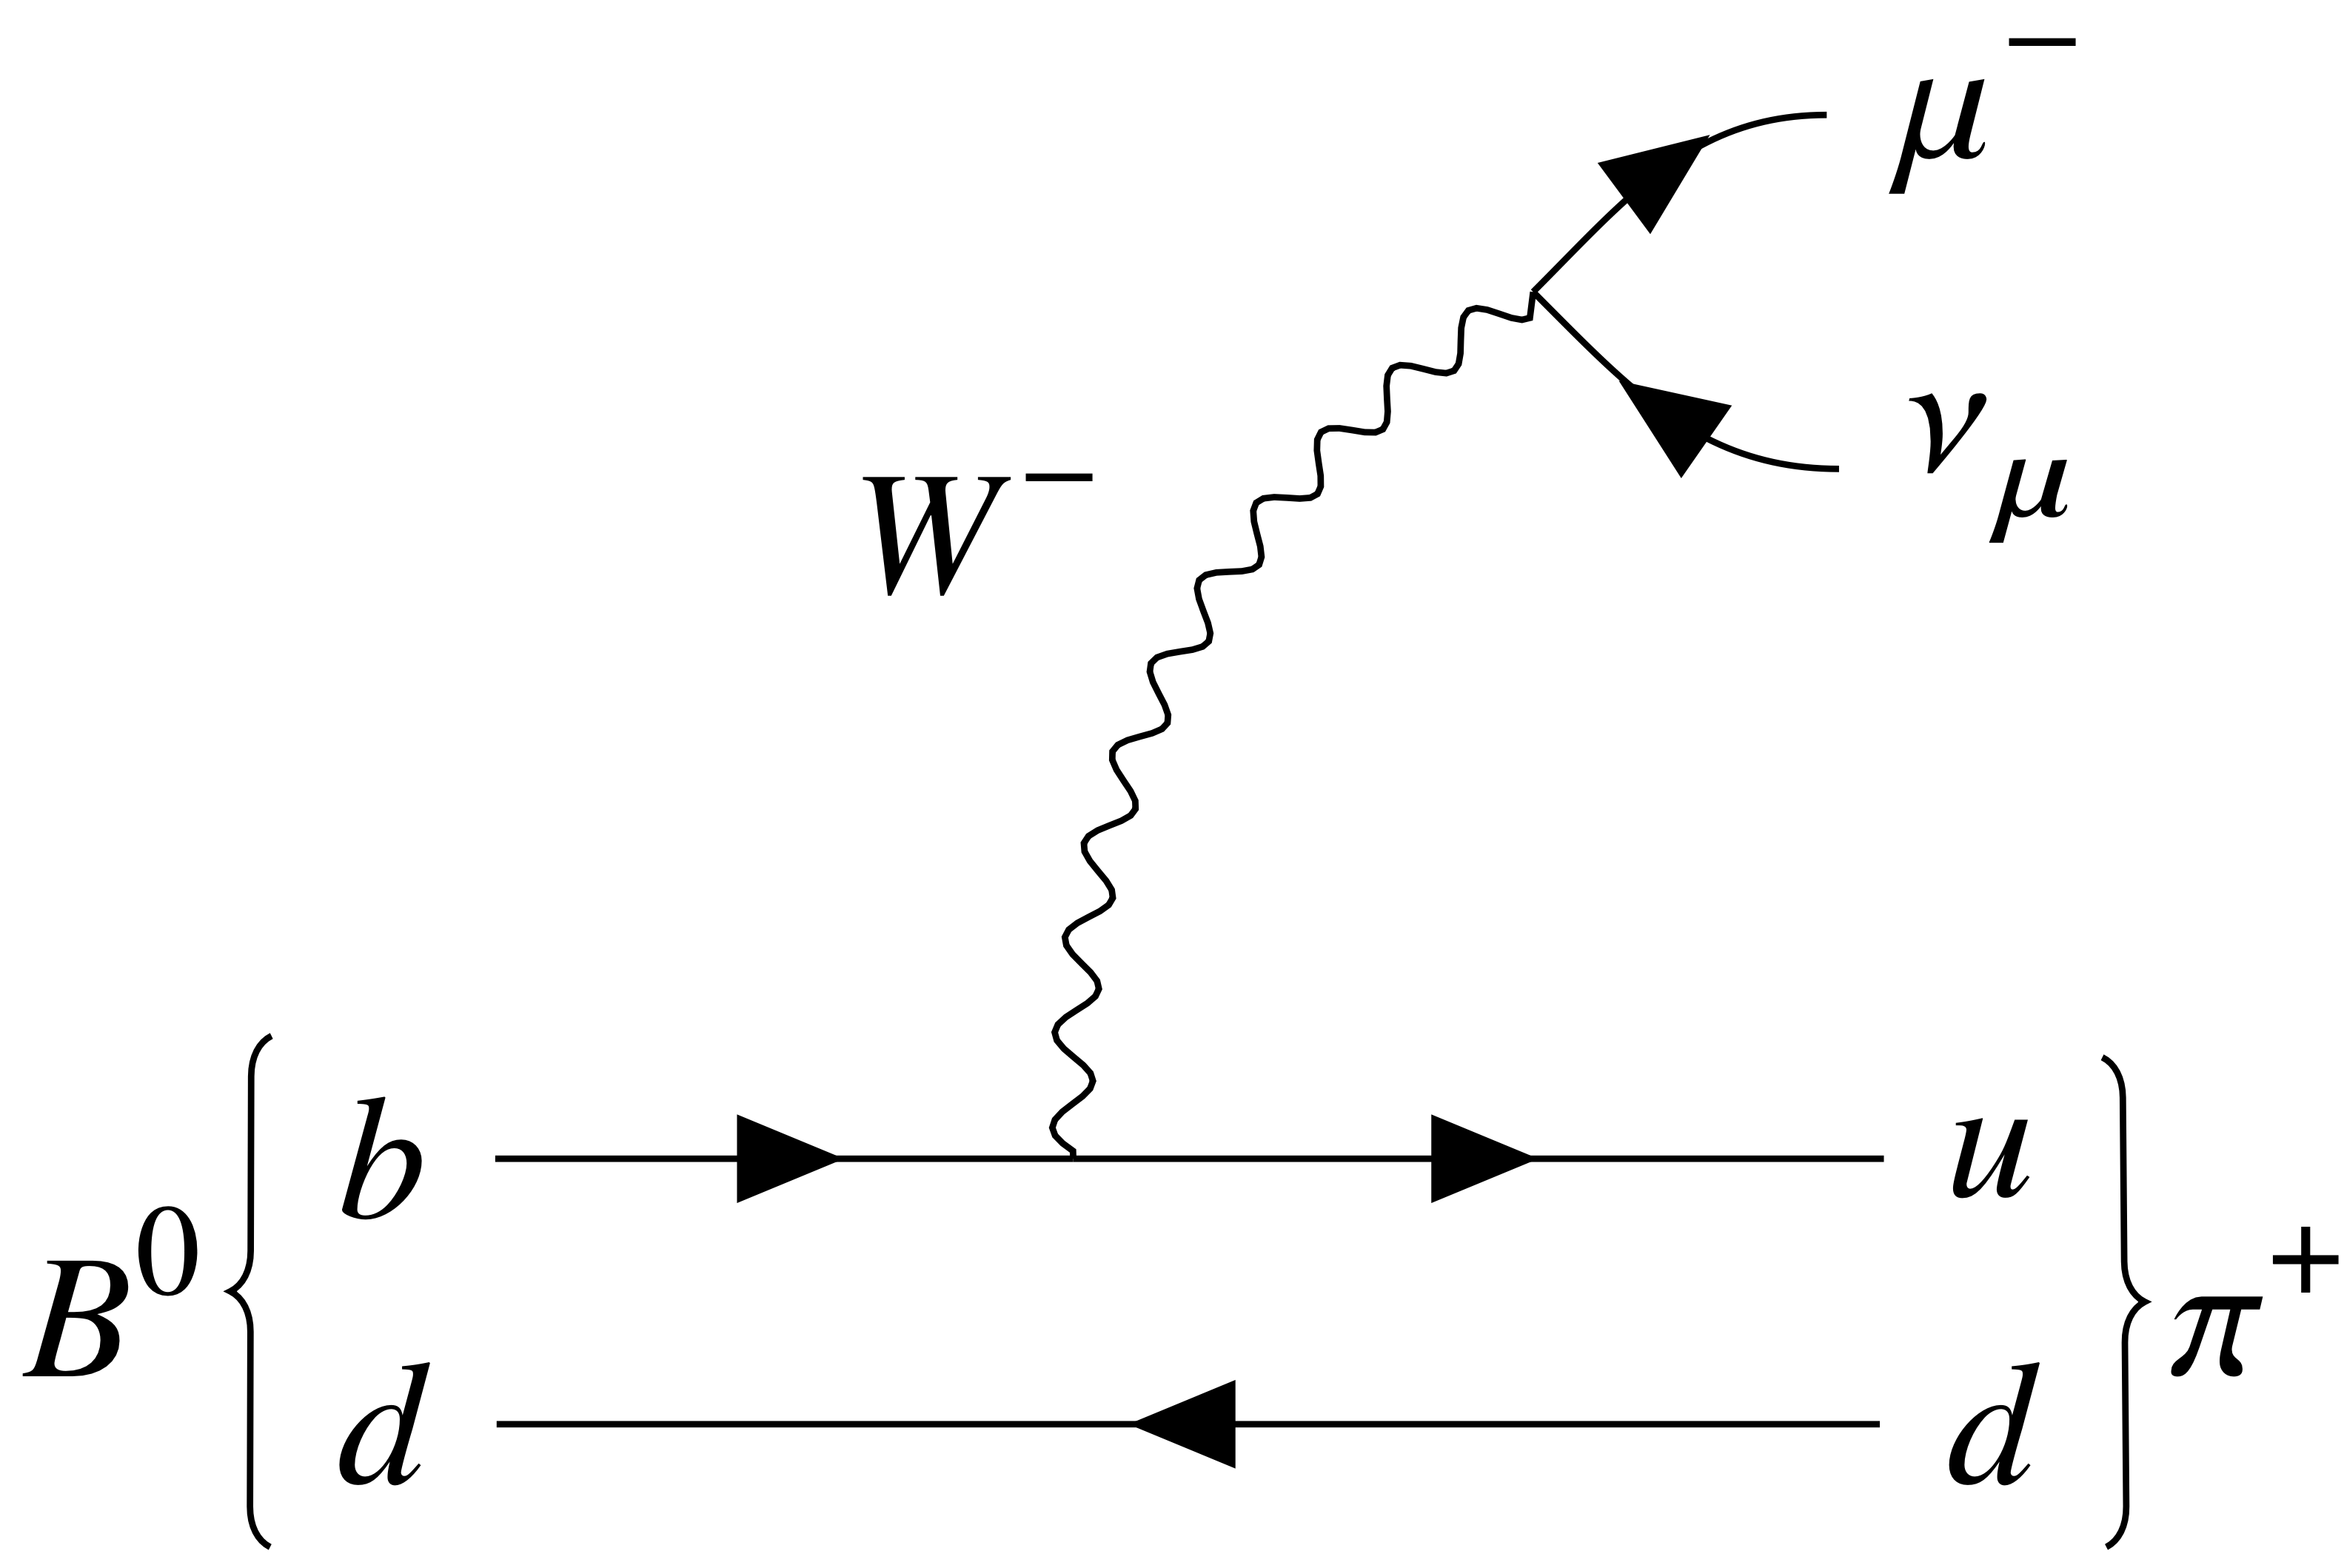
\includegraphics[width=0.4\textwidth]{semileptonic_b_decay}
  \caption{Feynman Diagram depicting a typical semi-leptonic decay of an Anti-$B^0$-meson containing a muon in the final state.}
  \label{fig:semileptonicDecay}
\end{figure}

Despite their limited branching ratio, muons from semi-leptonic heavy-flavor decays are valuable in complementing impact parameter- and vertex-based $b$-tagging methods. These muons typically exhibit higher transverse momentum compared to those from lighter hadron decays, as shown in figure \ref{fig:softMuon_pt}. This relates also to the fact that muons from $b$-decays tend to be more boosted transverse to the jet axis and therefore have a larger orthogonal projection $p_\text{T}^\text{rel}$ of the muon-\pt onto the jet axis. This is calculated by taking the perpendicular part of the three vector muon-momentum to the three-vector jet momentum. The term ``soft'' is derived from the fact that their \pt is smaller than that typically possessed by muons from electroweak boson decays, since they originate from a secondary process \citep{ATL-PHYS-PUB-2017-013}.
\begin{figure}[]
  \centering
  \subfigure[]{
    \includegraphics[width=0.45\textwidth]{softMuon_pt}
    \label{fig:softMuon_pt}
  }\hspace*{0.5cm}
  \subfigure[]{
    \includegraphics[width=0.45\textwidth]{softMuon_pTrel}
    \label{fig:softMuon_pTrel_sketch}
  }\\
  \subfigure[]{
    \includegraphics[width=0.49\textwidth]{softMuon_dR}
    \label{fig:softMuon_dR}
  }
  \caption{Kinematics of soft muons: \textbf{(a)} transverse momentum distribution, \textbf{(b)} relative transverse momentum ($p_\text{T}^\text{rel}$) indicative of muons from direct $b$-jet decays being more boosted transversely to the jet axis, and \textbf{(c)} $\Delta R$ distribution between soft muons and jets, normalized per flavor.}
  \label{fig:muonsForSMT}
\end{figure}



% ---------------------------
\section{Muon Selection}
\label{sec:MuonSelection}
%-------------------------------------------------------------------------------
The particle flow algorithm used to reconstruct small-$R$ jets described in section \ref{sec:particle_flow} does not include muons. To address this muons are associated to jets using the shrinking association \DeltaR cone as depicted in figure \ref{fig:shrinkCone}.
\begin{figure}[]
  \centering
  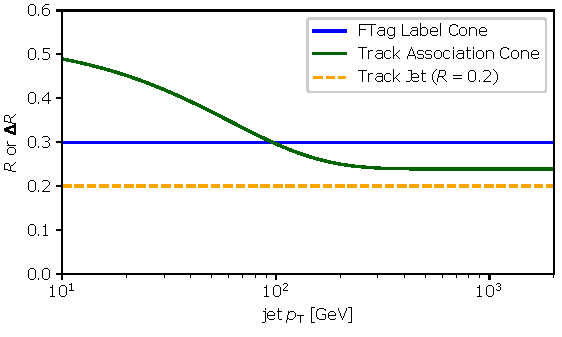
\includegraphics[width=0.5\textwidth]{shrinkCone}
  \caption{The shrinking particle association cone (\hexline{006401}) used to associate muons with a $\DeltaR_\mathrm{\mu, jet}$ smaller than the cone depending on the transverse momentum of the jet. Adopted from \citep{Jacobs:2697316}. }
  \label{fig:shrinkCone}
\end{figure}
Selected muons must be combined muons meaning they are reconstructed using both the inner detector and the muon spectrometer. The closest muon within $\DeltaR_\mathrm{\mu, jet} < 0.4$ to the jet axis is chosen provided it has a minimum \pt of \qty{4}{GeV}. This threshold is set as muon reconstruction below \qty{3}{GeV} is generally unreliable due to minimally ionizing particles losing approximately \qty{3}{GeV} in the ATLAS calorimeters \citep{expectedPerformanceAtlas}.

Truth studies revealed that most muons associated to jets result from secondary (non-prompt) decays of $c$- and $b$-hadrons as as evidenced in figure \ref{fig:muonTruth}(a). However this figure also reveals the introduction of $b$-tagging backgrounds since muons are also associated to light jets. These backgrounds predominantly arise from in flight decays of pions and kaons but also prompt muons from nearby $W$-boson decays and muons from light and strange mesons as shown in figure \ref{fig:muonTruth}(b).
\begin{figure}[]
  \centering
  \subfigure[]{
    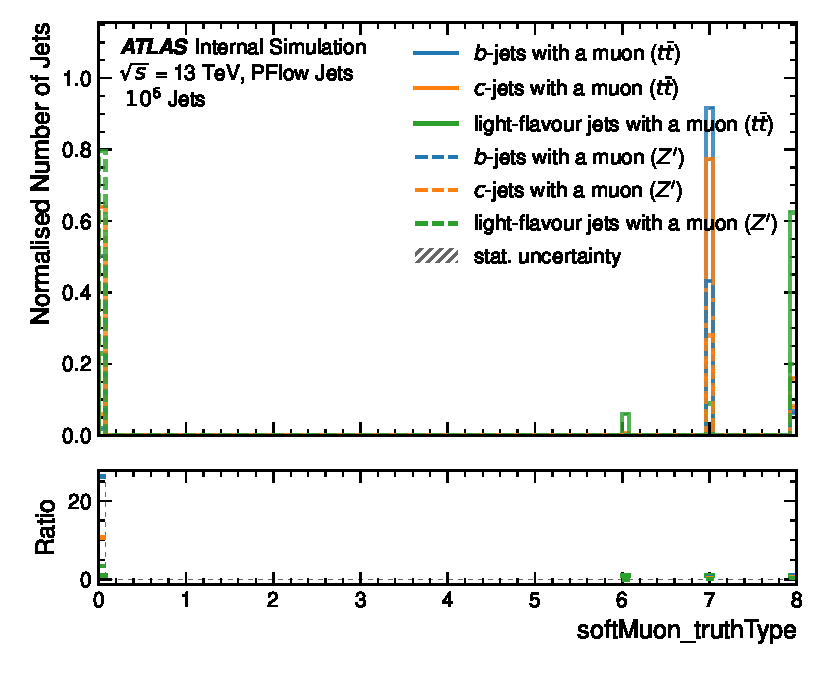
\includegraphics[width=0.47\textwidth]{softMuon_truthType_norm}
  }
  \subfigure[]{
    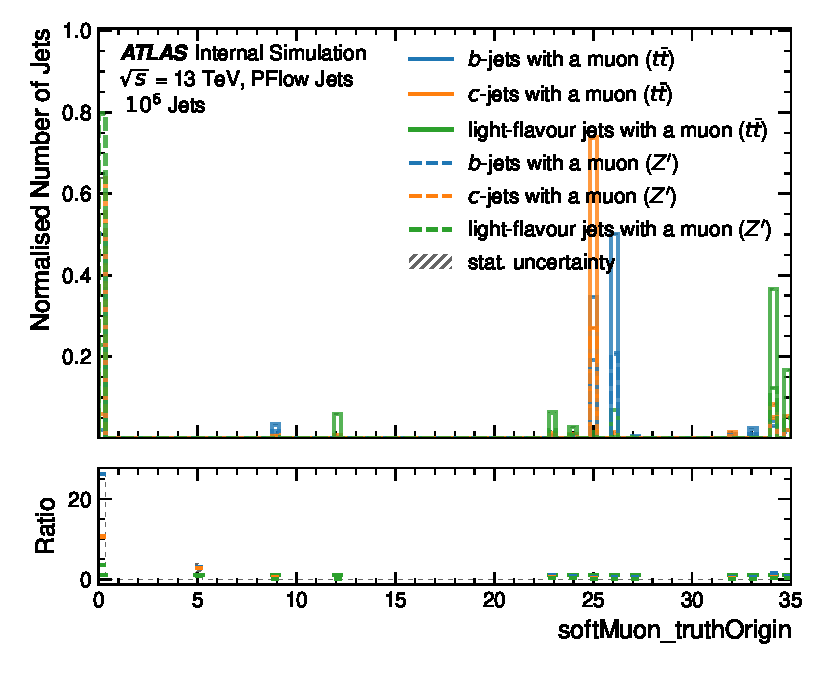
\includegraphics[width=0.47\textwidth]{softMuon_truthOrigin_norm}
  }
  \caption{Jet truth type (a) and truth origin (b) for jets with an associated muon normalized per flavor from $t\overline{t}$ and $Z'$ samples. Truth types: unclassified (0), prompt (6), non-prompt (7) and background muon (8). Truth origins: tau lepton decays (9), prompt muons from nearby W decays (12), light (23), strange (24), charm (25), bottom (26) mesons and in flight decays of pions (34) and kaons (35) according to the Monte Carlo truth classification \citep{mctruthclassification}.}
  \label{fig:muonTruth}
\end{figure}
Table \ref{tab:MuonJetFlavors} shows the proportion of jets with an associated muon for each flavor. Approximately \qty{15}{\percent} of $b$-jets and around \qty{1}{\percent} of both light and tau jets have an associated muon.
\begin{table}[]
  \caption{Fraction of associated muons per flavor. The large fraction for $b$-jets compared to the other flavors is the reason why muons are a useful discriminator for $b$-tagging. }
  \label{tab:MuonJetFlavors}
  \centering
  \begin{tabular}{ l c }
    \hline
    Jet flavor & Fraction of jets with an associated muon \\
    \hline
    light      & 0.0134                                   \\
    c          & 0.0472                                   \\
    b          & 0.1490                                   \\
    tau        & 0.0138                                   \\
    \hline
  \end{tabular}
\end{table}
Figure \ref{fig:muon_2d_truth} visualizes the amount of fake muons in $b$-jets with an associated muons depending on the jet- and muon-\pt. A notable trend is that $b$-jets with low momentum tend to have low momentum muons. Falsely associated muons become more common at high jet momentum and low muon momentum.
\begin{figure}[]
  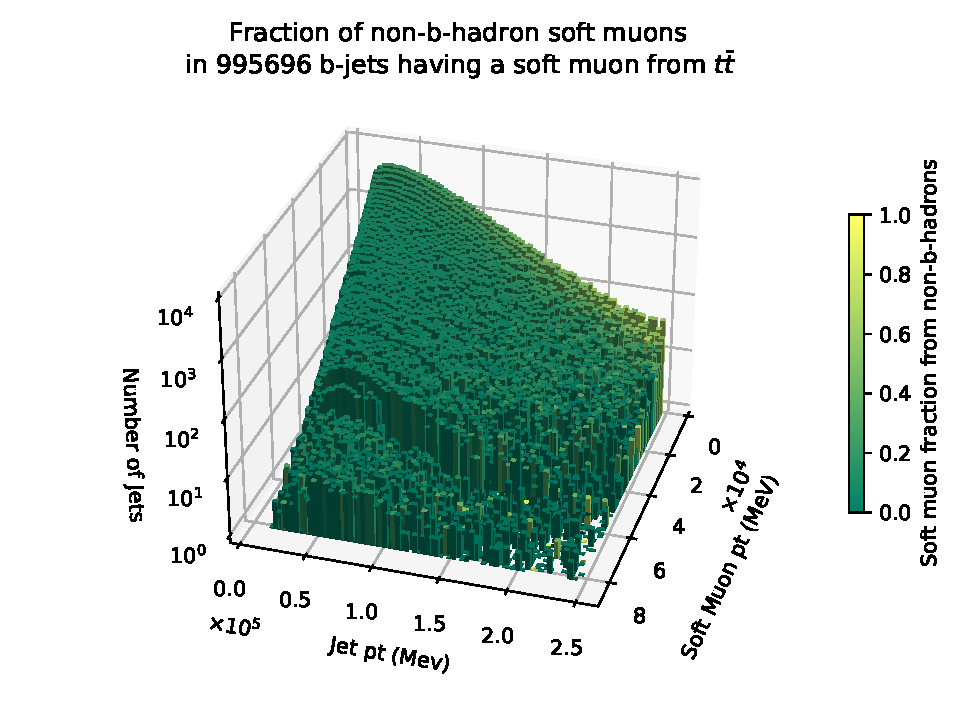
\includegraphics[width=1\textwidth]{muon_2d_truth_ttbar}
  \caption{2D histograms of $p_\mathrm{T}^\mathrm{jet}$ and $p_\mathrm{T}^\mathrm{muon}$ for $t\bar{t}$ selected on $b$-jets only. The colorbar is the fraction of muons that do not originate from b-hadrons. The distribution is actually smooth although some irregularities are visible which is due to a bug in the plotting library.}
  \label{fig:muon_2d_truth}
\end{figure}



\section{Soft Muon Variables}
\label{sec:SoftMuonVariables}
The soft muon variables are selected based on their $b$-tagging discrimination power. The impact parameters of jets as described in section \ref{sec:b_tagging} are determined with the three dimensional impact parameter algorithm (IP3D) detailed in \citep{ATL-PHYS-PUB-2017-013} and are shown in figure \ref{fig:softMuon_ip3dD0}-\ref{fig:softMuon_ip3dZ0Significance}.
\begin{figure}[]
  \centering
  \subfigure[]{
    \includegraphics[width=0.47\textwidth]{softMuon_ip3dD0}
    \label{fig:softMuon_ip3dD0}
  }
  \subfigure[]{
    \includegraphics[width=0.47\textwidth]{softMuon_ip3dZ0}
    \label{fig:softMuon_ip3dZ0}
  }
  \\
  \subfigure[]{
    \includegraphics[width=0.47\textwidth]{softMuon_ip3dD0Significance}
    \label{fig:softMuon_ip3dD0Significance}
  }
  \subfigure[]{
    \includegraphics[width=0.47\textwidth]{softMuon_ip3dZ0Significance}
    \label{fig:softMuon_ip3dZ0Significance}
  }
  \caption{Impact parameters of the soft muon retrieved with the IP3D algorithm \citep{ATL-PHYS-PUB-2017-013}, normalized per flavor.}
  \label{fig:softMuonKinematics}
\end{figure}
In addition variables are used to reject muons from in flight decays of Kaons and Pions \citep{ATLAS-CONF-2020-030}. The Scattering Neighbor Significance measures if the track of a particle has kinks that could be a sign of an additional decay. By connecting neighboring detector hits along the track with straight lines and measuring the angles between adjacent lines the Scattering Neighbor Significance is obtained by taking the maximum of the angle divided by its uncertainty. In figure \ref{fig:softMuon_scatteringNeighbourSignificance} light jets therefore tend to have larger values as they have a smaller \pt (cf. figure \ref{fig:softMuon_pt}). Another variable to identify possible background sources is the Momentum Balance Significance. It calculates the difference of the muon-\pt determined with the inner detector with the one from the muon spectrometer and corrects it for energy deposits in the calorimeters. This would be zero in figure \ref{fig:softMuon_momentumBalanceSignificance} for a perfect energy loss correction and if the muon did not arise from an in flight decay. Furthermore there is the curvature comparison between inner detector (ID) and the one from the muon spectrometer (MS) termed q over p ratio: $(q/p)_\mathrm{ID}\, \bm{/}\, (q/p)_\mathrm{MS}$ in figure \ref{fig:softMuon_qOverPratio}.

\begin{figure}[]
  \centering
  \subfigure[]{
    \includegraphics[width=0.47\textwidth]{softMuon_scatteringNeighbourSignificance}
    \label{fig:softMuon_scatteringNeighbourSignificance}
  }
  \subfigure[]{
    \includegraphics[width=0.47\textwidth]{softMuon_momentumBalanceSignificance}
    \label{fig:softMuon_momentumBalanceSignificance}
  }
  \\
  \subfigure[]{
    \includegraphics[width=0.47\textwidth]{softMuon_qOverPratio}
    \label{fig:softMuon_qOverPratio}
  }
  \caption{Variables to reject light jet background. Description in section \ref{sec:SoftMuonVariables}.}
  \label{fig:softMuonVariables2}
\end{figure}


\section{Neural Network Training}
For all trainings the Umami neural network training framework \citep{Froch:2857164} is used with \ttbar and \Zprime Monte Carlo samples described in \citep{ATL-PHYS-PUB-2017-013}. \Zprime is a hypothetical particle used here to enhance the statistics at larger jet-\pt>$\SI{250}{GeV}$. For the training both \ttbar and \Zprime samples are merged and resampled to make the \pt and $\eta$ distributions appear the same for all flavors. This is done to allow for a fair training between flavor categories, as the kinematic regimes are neither over- nor under-represented between flavors when the neural network is trained. The flavor composition of jets can be seen before and after applying the resampling in figure \ref{fig:resampling}. A total of \qty{23.6e6}{jets} are used with \qty{3.9e6}{jets} (\qty{16.6}{\percent}) having an associated soft muon.
\begin{figure}
  \centering
  \subfigure[]{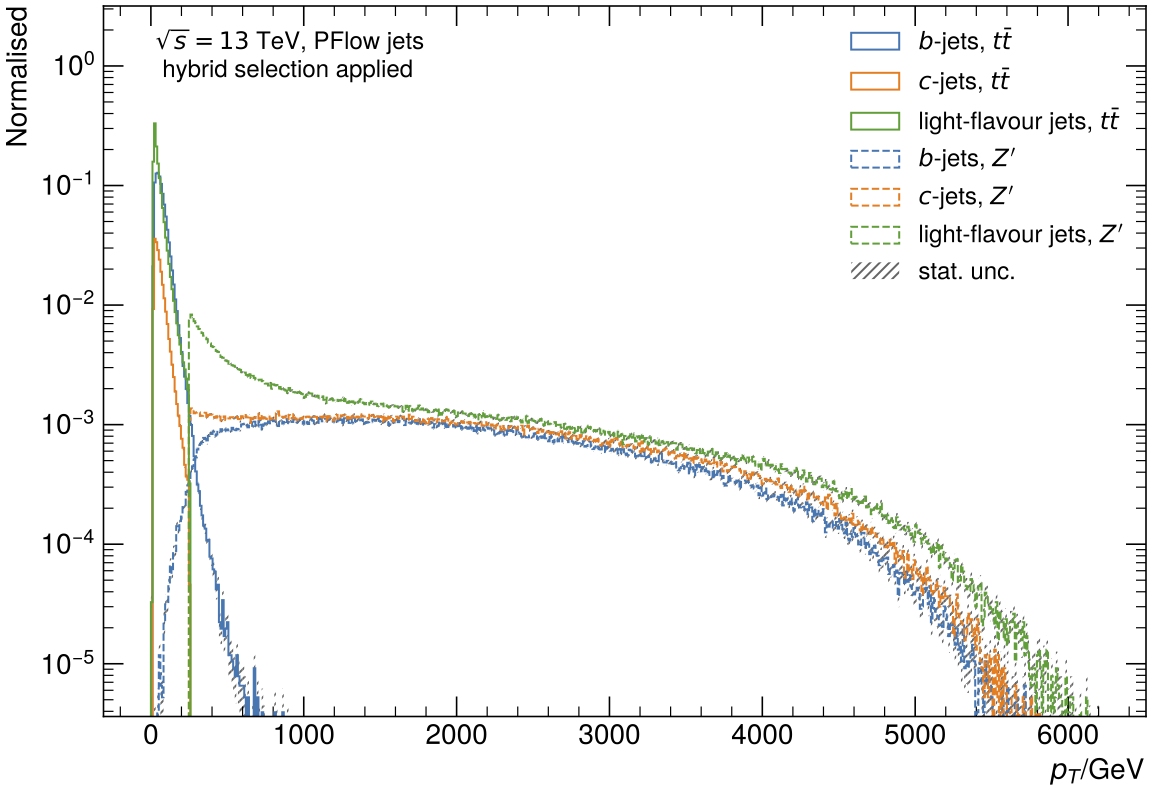
\includegraphics[width=.8\textwidth]{pt_btagJes-cut_spectrum}}\\
  \subfigure[]{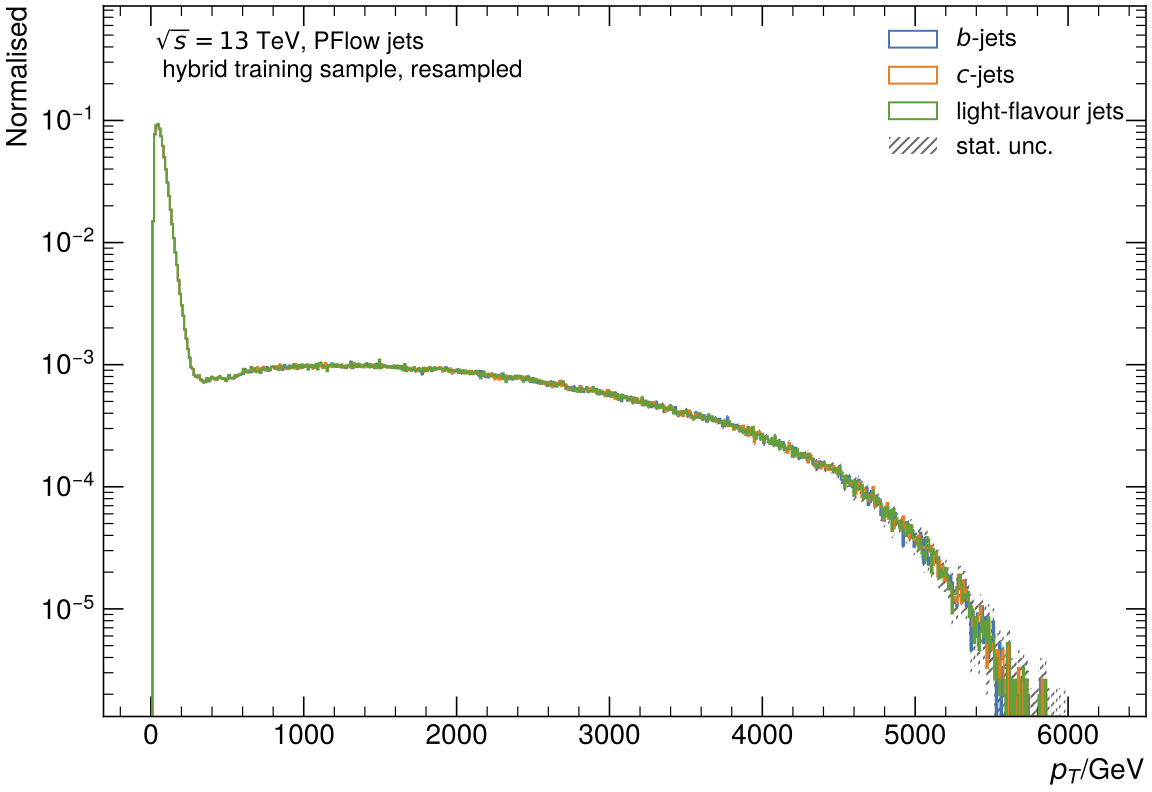
\includegraphics[width=.8\textwidth]{pt_btagJes-downsampled}}
  \caption[]{Jet-\pt per flavor normalized to unity for \ttbar and \Zprime samples \textbf{(a)} before and \textbf{(b)} after resampling. Adopted from \citep{umamiDocs}.}
  \label{fig:resampling}
\end{figure}


\section{Adding muons to $b$-tagging algorithms}\label{sec:add_muons}
Current $b$-tagging algorithms in use are deep feed-forward neural networks with the prefix \ac{dl1} that assign a probability score ($p_\mathrm{b}, p_\mathrm{c}, p_\mathrm{light}$) to a jet depending on its flavor content. Depending on the strategy used to introduce additional tracking information associated with the jet it can become DL1r if the outputs of the RNNIP (Recurrent Neural Network Impact Parameter) \citep{Gilles:2806947} tagger or DL1d if the outputs of the \ac{dips} \citep{ATL-PHYS-PUB-2020-014} tagger are added as inputs to \ac{dl1}. The outputs of these taggers are then combined into a single signal to background ratio variable, the discriminant, defined as
\begin{equation}
  \mathrm{D}=\ln\left(\frac{p_b}{f_c \cdot p_c + (1-f_c)\cdot p_\mathrm{light} }\right).
\end{equation}
$f_c$ is the fraction of charm jets in the background and can be used to tune the importance of the different background classes ($\sum f_\mathrm{bkg} =1$).
Figure \ref{fig:scores_comparison_DL1d_to_DL1dmu} illustrates the discriminant of DL1d in comparison to the DL1dmu tagger, which will be discussed later.
\begin{figure}[]
  \centering
  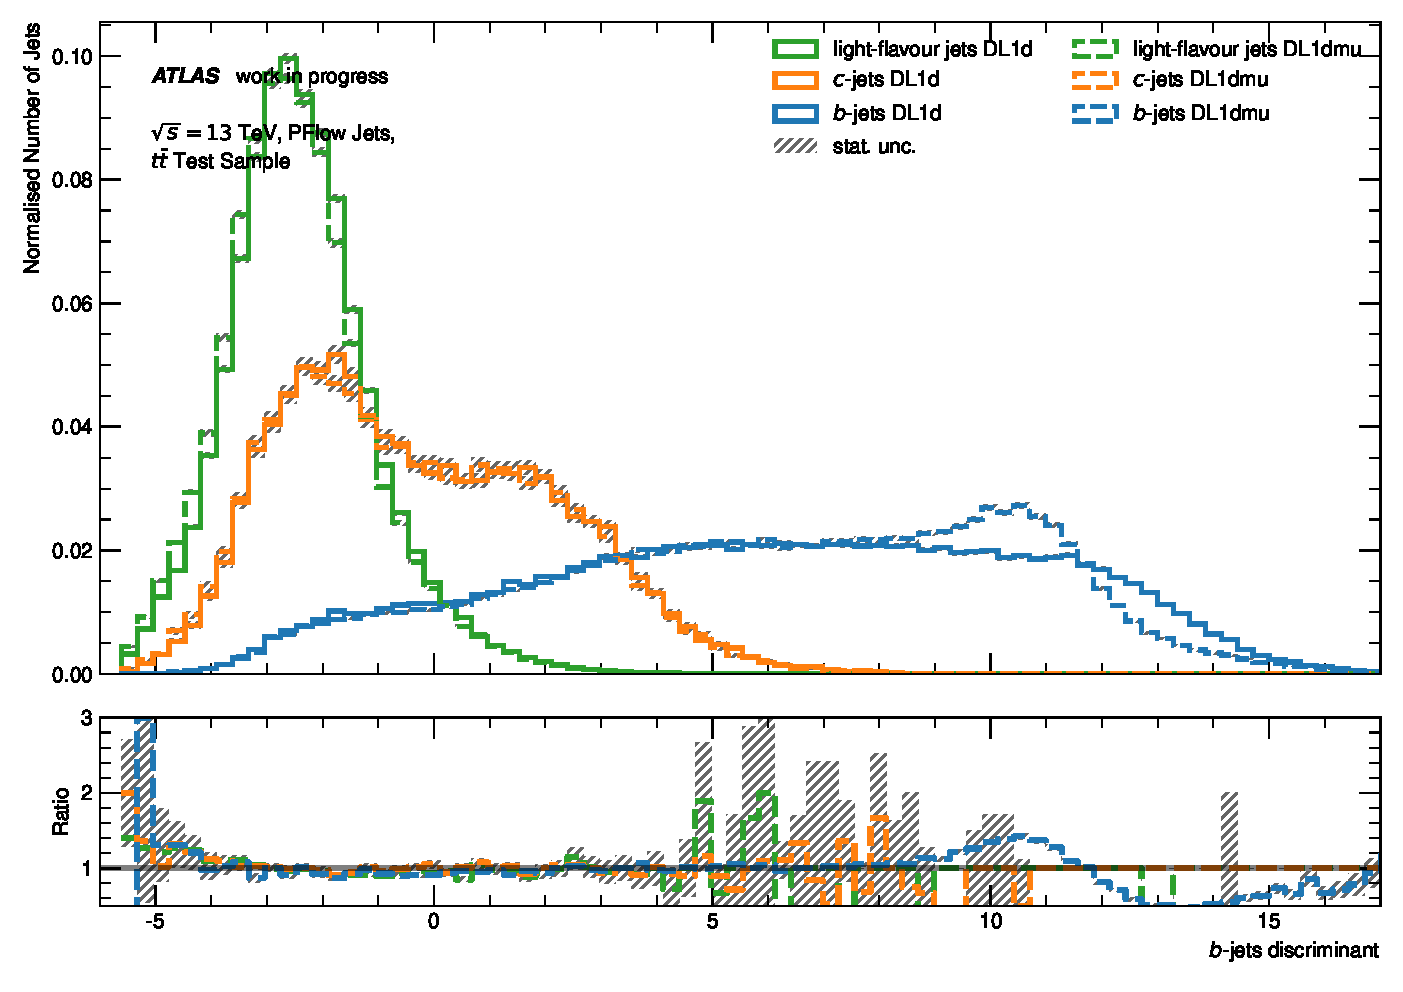
\includegraphics[width=0.7\textwidth]{scores_comparison_DL1d_to_DL1dmu}
  \caption{Discriminant comparison between DL1d ($\bm{\diagup$}) and DL1dmu (\textbf{- -}). Enhanced model performance is indicated by greater visual separation between the classes.}
  \label{fig:scores_comparison_DL1d_to_DL1dmu}
\end{figure}

Information of the selected muon variables are added to these tracking information inclusive taggers as additional inputs. For a performance reference point initial trainings of DL1r were conducted and two ways of introducing the muon information were explored. The first refers to an approach where the muon variables itself were used to train an additional neural network called the \ac{smt} with architecture: (soft muon input variables) $\rightarrow$ 3 hidden layers (100, 20, 10) $\rightarrow (p_\text{b}, p_\text{c}, p_\text{light})$. The output scores of the \ac{smt} are then added as inputs to the \ac{dl1} training. The tagger resulting from this method will be referred to as DL1rSMT. In a second approach the muon variables were added directly as inputs to the DL1r training and are denoted as DL1rmu.

\section{Performance evaluation}
A retraining of the DL1r or DL1d tagger serve in all cases as performance reference point against which other models are compared to. As a typical evaluation metric \ac{roc} curves are used to evaluate a classifier. In these curves the true positive rate (rate at which the classifier identifies correctly what it should identify) is plotted against the false positive rate (rate at which the classifier identifies falsely what it should identify). The first translates here into the $b$-jet efficiency. It corresponds to integrating from right to left in figure \ref{fig:scores_comparison_DL1d_to_DL1dmu} for a desired $b$-jet efficiency. The latter (false positive rate) will be plotted inversely here as rejection instead of as efficiency (1/$\epsilon_\mathrm{flavor}$.) For the case at hand the performance increases if the curve moves to the upper right corner, as the model can reject more background for a designated $b$-jet efficiency. If the \ac{roc} curve of a classifier would be a \qty{45}{\degree} line the classifier is of no use as there would be always a \qty{50}{\percent} chance to correctly or falsely identify a property of interest, essentially performing no better than random chance.

\section{DL1rmu vs. DL1rSMT}
\ac{roc} curves comparing performances of DL1r, DL1rmu and DL1rSMT, detailed in \ref{sec:add_muons} are shown in figure \ref{fig:DL1rmu_vs_DL1r_SMT_tt} and \ref{fig:DL1rmu_vs_DL1r_SMT_z} which shows a \qty{25}{\percent} improvement in the light flavor jet rejection and a \qty{10}{\percent} $c$-flavor jet rejection upon introducing muon information.  Since adding the soft muon variables to the inputs of DL1r/DL1d results in fewer technical interdependencies and also allows DL1r to figure out potential correlations to other variables, it was decided to default to this option.

\begin{figure}[]
  \centering
  \subfigure[]{
    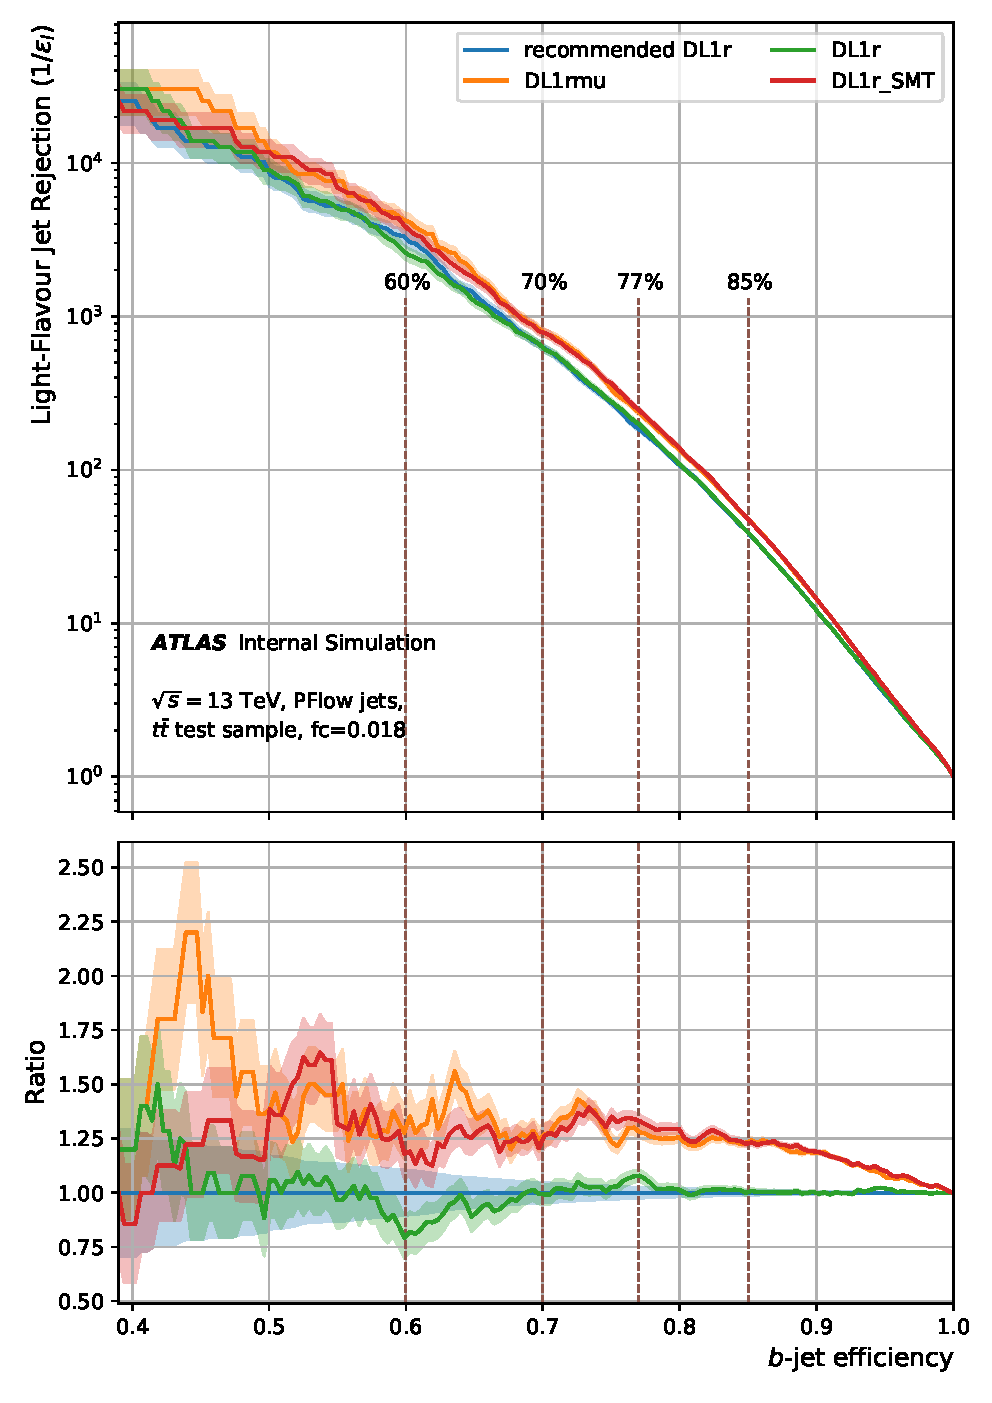
\includegraphics[width=0.477\textwidth]{DL1r_light_flavour_ttbar_229}
    \label{fig:DL1rmu_vs_DL1r_SMTa}
  }
  \subfigure[]{
    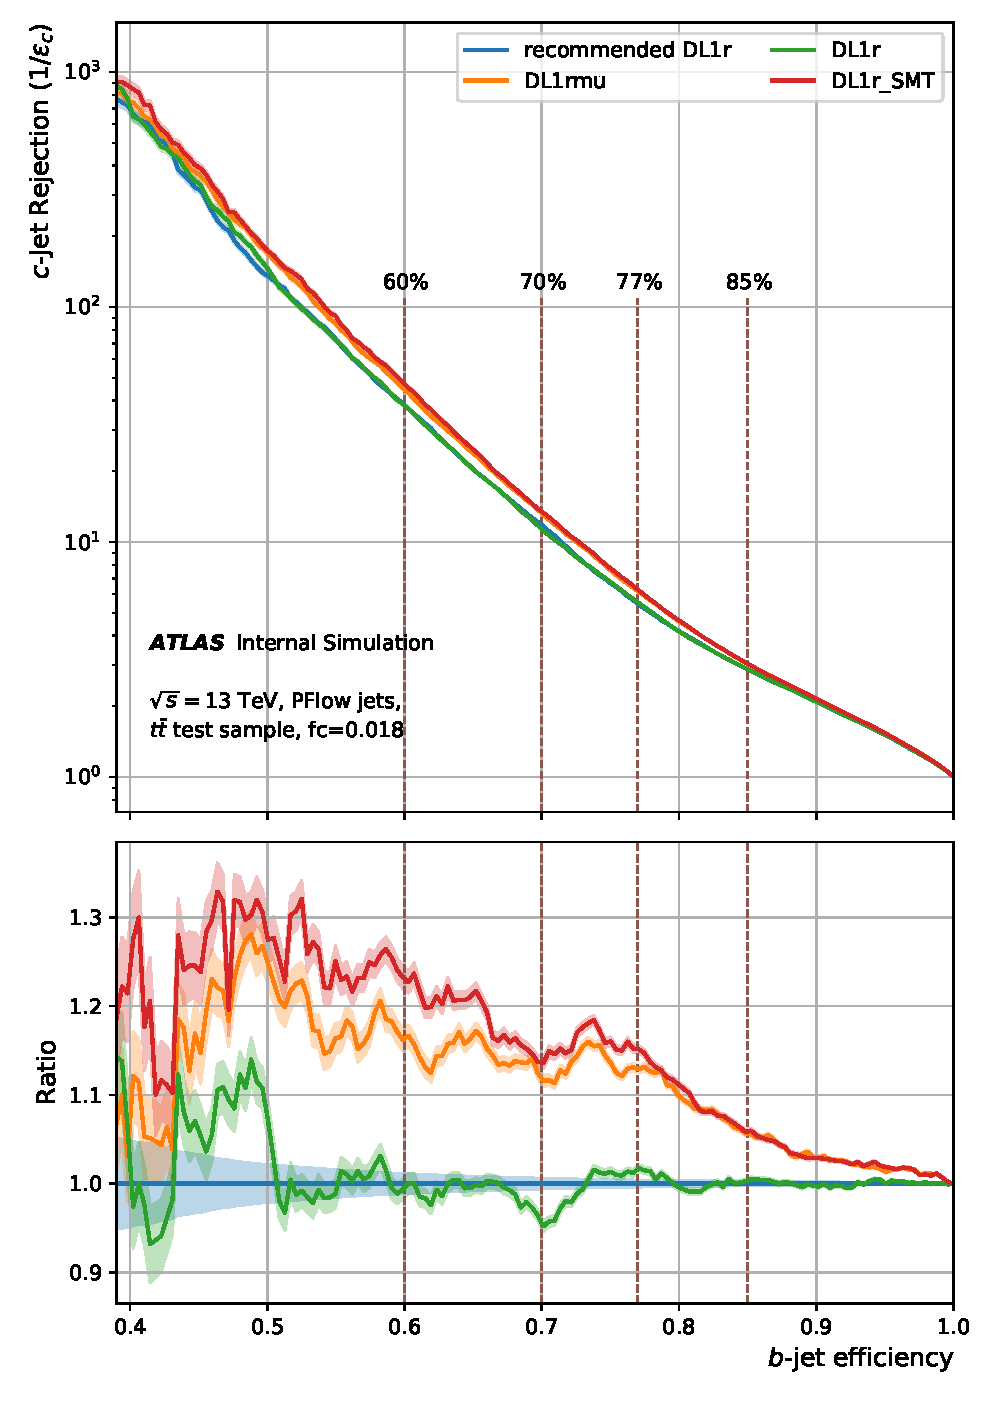
\includegraphics[width=0.477\textwidth]{DL1r_c_flavour_ttbar_229}
    \label{fig:DL1rmu_vs_DL1r_SMTb}
  }
  \caption{ROC curves of different trainings. Official performance of DL1r (\hexline{1F77B5}), Trainings: DL1r (\hexline{549F41}), DL1rmu (\hexline{EF8636}) adds the soft muon variables to the inputs variables of DL1r,  DL1rSMT (\hexline{C53A32}) adds the outputs from the standalone Soft Muon Tagger neural network to the inputs of DL1r evaluated on \ttbar. }
  \label{fig:DL1rmu_vs_DL1r_SMT_tt}
\end{figure}

\begin{figure}[]
  \centering
  \subfigure[]{
    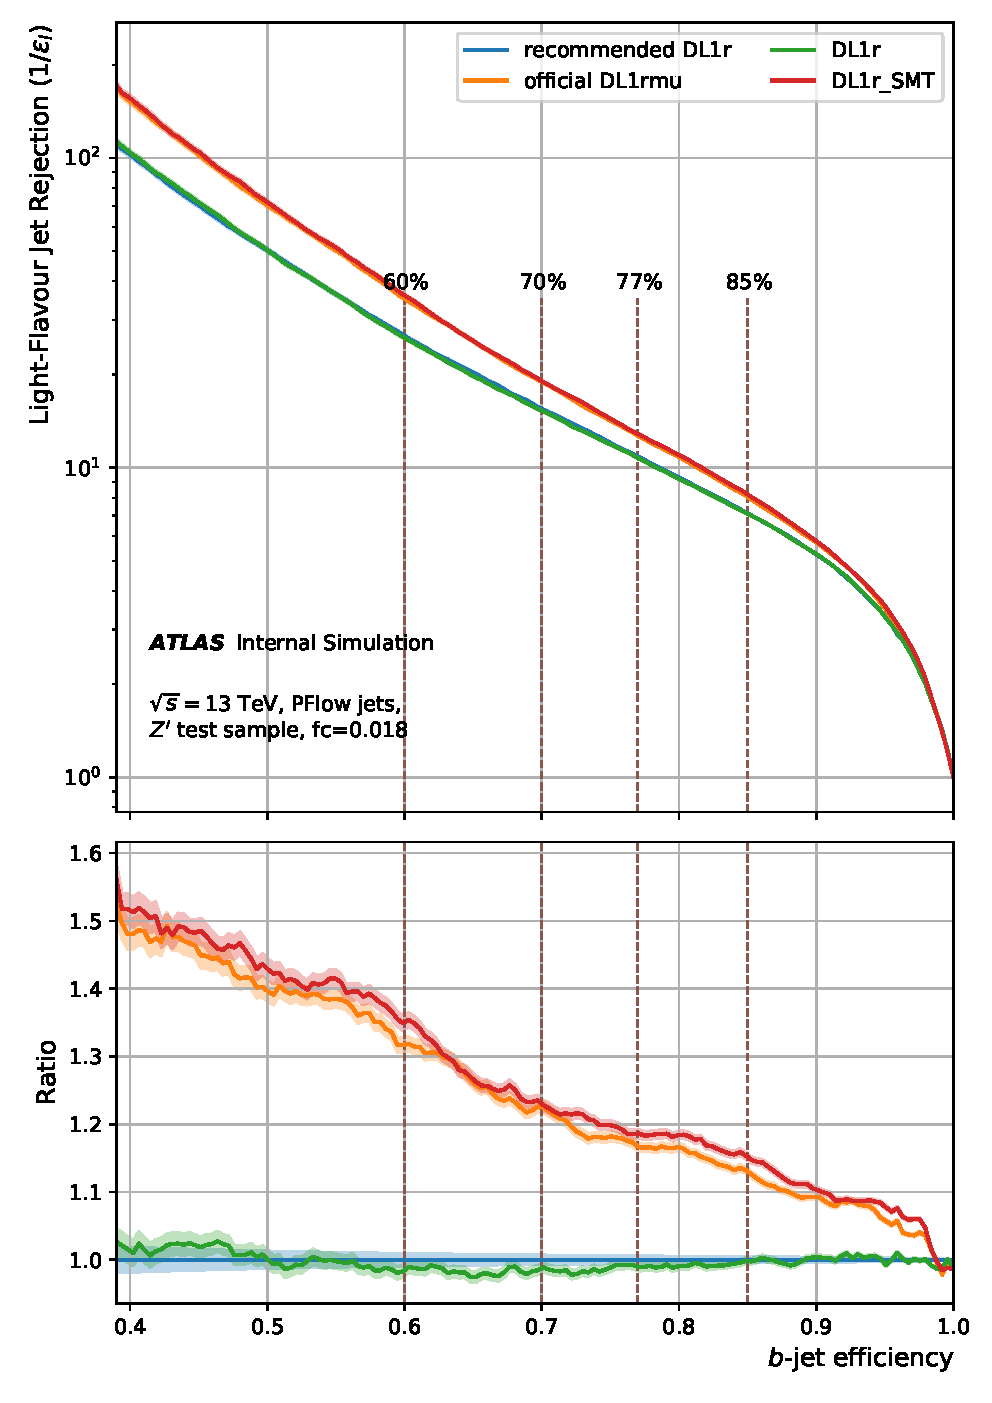
\includegraphics[width=0.477\textwidth]{DL1r_light_flavour_zpext_229}
    \label{fig:DL1rmu_vs_DL1r_SMTc}
  }
  \subfigure[]{
    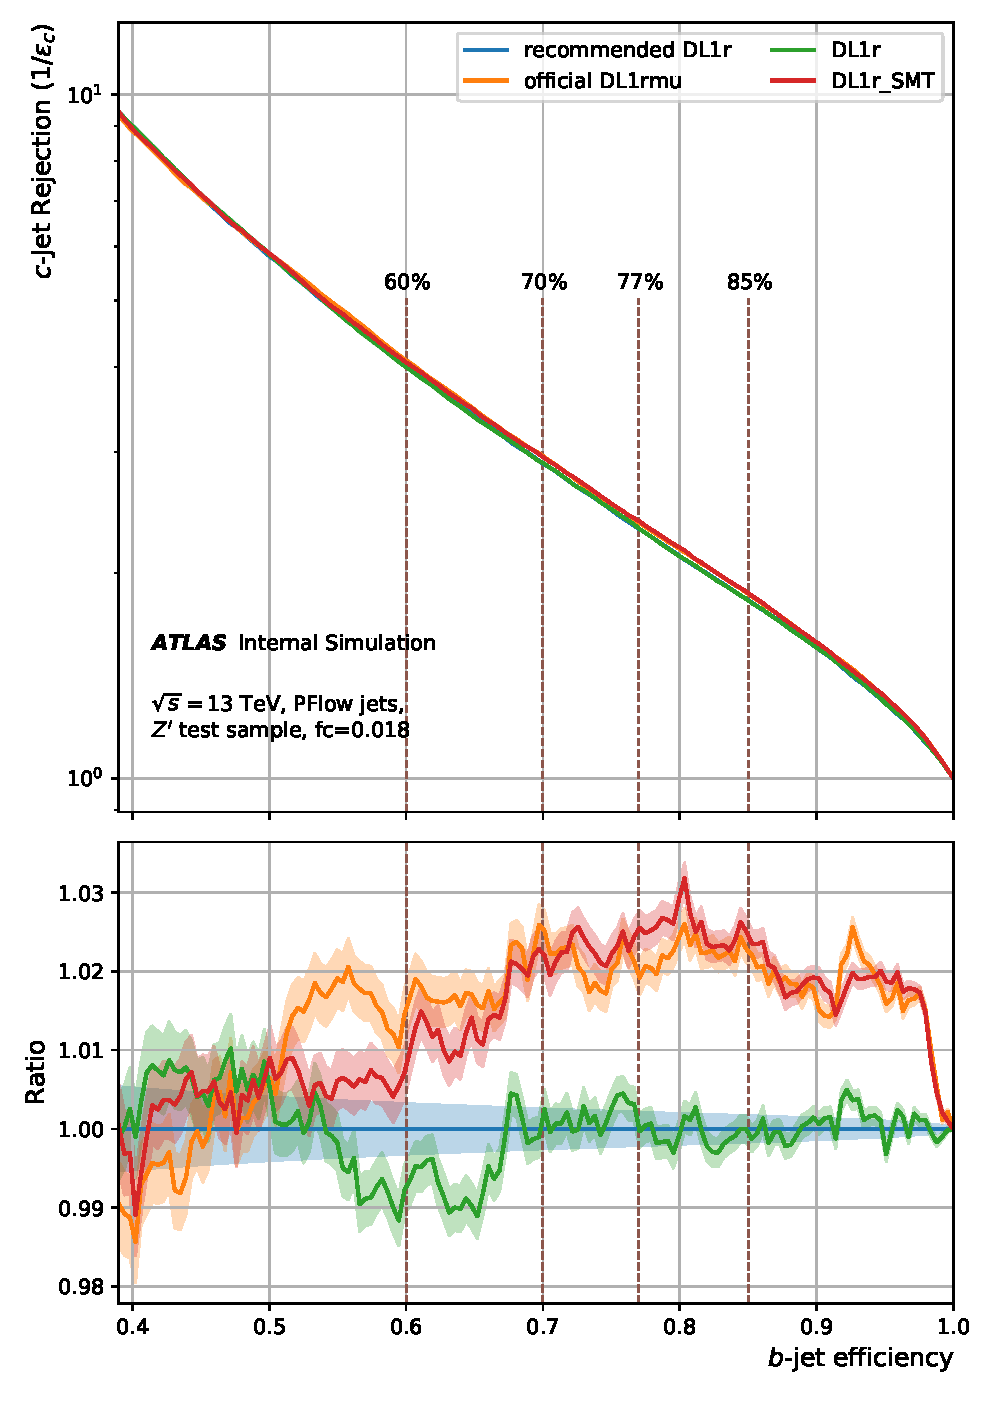
\includegraphics[width=0.477\textwidth]{DL1r_c_flavour_zpext_229}
    \label{fig:DL1rmu_vs_DL1r_SMTd}
  }
  \caption{ROC curves of different trainings. Official performance of DL1r (\hexline{1F77B5}), Trainings: DL1r (\hexline{549F41}), DL1rmu (\hexline{EF8636}) adds the soft muon variables to the inputs variables of DL1r,  DL1rSMT (\hexline{C53A32}) adds the outputs from the standalone Soft Muon Tagger neural network to the inputs of DL1r evaluated on \Zprime. }
  \label{fig:DL1rmu_vs_DL1r_SMT_z}
\end{figure}



\section{Additional soft muon variables}
The full potential of muons were explored phenomenologically by successively adding input variables of four different classes to \ac{dl1}. New inputs are categorized into variables related to quality criteria used by the \ac{mcp} group, number of hits in the various subdetectors of the inner detector and of course the tracking information from \ac{dips} and mentioned \ac{smt} variables as detailed in \ref{sec:SoftMuonVariables}. Results are shown in section \ref{sec:dl1d_results}

The different variations of input variables are shown in table \ref{tab:smtAbbreviations} and \ref{tab:DL1dModels} while figures \ref{fig:smt_vars_1}-\ref{fig:smt_vars_7} show their distributions per flavor. Table \ref{tab:smtAbbreviations} is a reduced version of available variables since some of them did not display any flavor discrimination power. A detailed explanation and modeling of these variables can be found in \citep{Assamagan:1099953,Bugge:2665711}.

\begin{table}[]
  % \sisetup{group-minimum-digits=4}
  \caption{Abbreviations for the different sets of variables}%
  \label{tab:smtAbbreviations}
  \centering
  \resizebox{0.97\textwidth}{!}{
    \begin{tabular}{c|l|l
      }
      \hline
      Abbreviation                & SMT                              & Hits                                      \\
      \hline
      \multirow{15}{*}{Soft Muon} & \pt                              & numberOfInnermostPixelLayerHits           \\
                                  & \DeltaR                          & numberOfInnermostPixelLayerSplitHits      \\
                                  & q over p ratio                   & numberOfInnermostPixelLayerSharedHis      \\
                                  & Momentum Balance Significance    & numberOfInnermostPixelLayerOutliers       \\
                                  & Scattering Neighbor Significance & numberOfNextToInnermostPixelLayerHits     \\
                                  & \ptrel                           & numberOfNextToInnermostPixelLayerOutliers \\
                                  & ip3dD0                           & numberOfPixelHits                         \\
                                  & ip3dZ0                           & numberOfPixelSplitHits                    \\
      Variables                   & ip3dD0 Significance              & numberOfPixelSharedHits                   \\
                                  & ip3dZ0 Significance              & numberOfPixelSpoiltHits                   \\
                                  & isDefaults                       & numberOfPixelHoles                        \\
                                  &                                  & numberOfSCTHits                           \\
                                  &                                  & numberOfSCTSharedHits                     \\
                                  &                                  & numberOfSCTHoles                          \\
                                  &                                  & expectInnermostPixelLayerHits             \\
                                  &                                  & expectNextToInnermostPixelLayerHits       \\

      \hline
      Abbreviation                & MCP                              & dips                                      \\
      \hline
      \multirow{9}{*}{Soft Muon}  & segmentDeltaEta                  & dipsLoose20210729 pb                      \\
                                  & segmentDeltaPhi                  & dipsLoose20210729 pc                      \\
                                  & ParamEnergyLoss                  & dipsLoose20210729 pu                      \\
                                  & ParamEnergyLossSigmaPlus         &                                           \\
                                  & ParamEnergyLossSigmaMinus        &                                           \\
      Variables                   & MeasEnergyLoss                   &                                           \\
                                  & MeasEnergyLossSigma              &                                           \\
                                  & CaloMuonScore                    &                                           \\
                                  & Muon Quality                     &                                           \\
                                  & Nr. of Associated Muons          &                                           \\
                                  & CaloMuonIDTag                    &                                           \\
      \hline
    \end{tabular}
  }
\end{table}

\begin{table}[]
  % \sisetup{group-minimum-digits=4}
  \caption{Variables used in the different trainings of DL1d}%
  \label{tab:DL1dModels}
  \centering

  \begin{tabular}{c| llll
    }
    \hline
    Model                            & DL1d & DL1dmu & DL1dmu add hits & DL1dmu add all \\
    \hline
    \multirow{4}{*}{Input Variables} & DL1  & DL1    & DL1             & DL1            \\
                                     & dips & dips   & dips            & dips           \\
                                     &      & SMT    & SMT             & SMT            \\
                                     &      &        & Hits            & Hits           \\
                                     &      &        &                 & MCP            \\
    \hline
  \end{tabular}
\end{table}

\newcommand\plotsize{0.30}
\begin{figure}[]
    \centering
    \subfigure[]{
        \includegraphics[width=\plotsize\textwidth]{input_vars_smt_ttbar_zpext/softMuon_pt}
    }
    \subfigure[]{
        \includegraphics[width=\plotsize\textwidth]{input_vars_smt_ttbar_zpext/softMuon_dR}
    }
    \subfigure[]{
        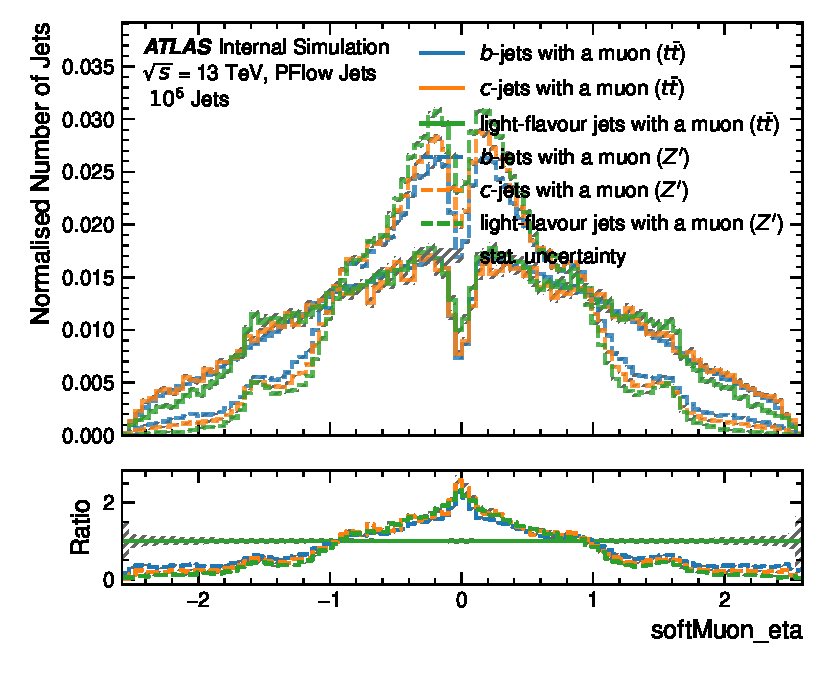
\includegraphics[width=\plotsize\textwidth]{input_vars_smt_ttbar_zpext/softMuon_eta}
    }\\
    \subfigure[]{
        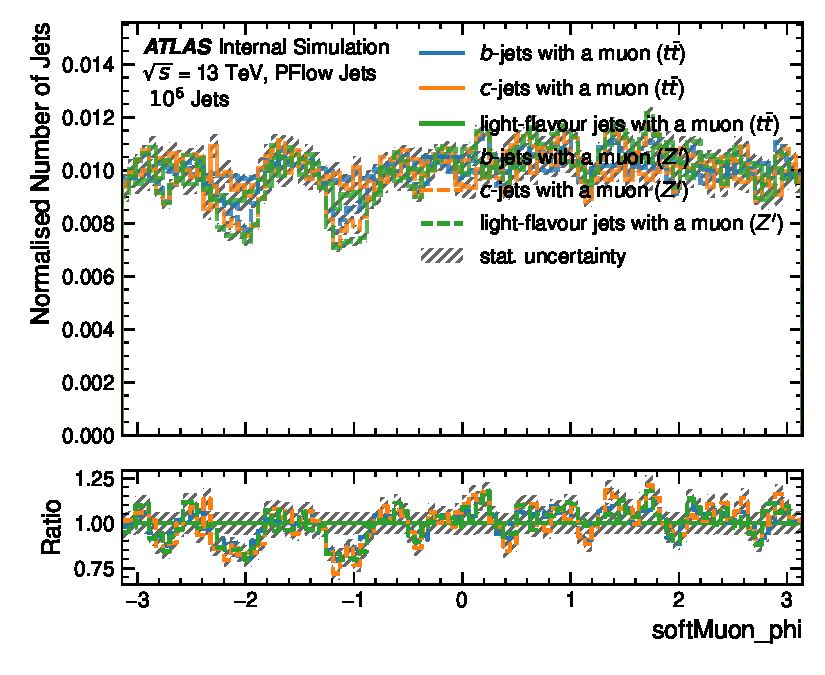
\includegraphics[width=\plotsize\textwidth]{input_vars_smt_ttbar_zpext/softMuon_phi}
    }
    \subfigure[]{
        \includegraphics[width=\plotsize\textwidth]{input_vars_smt_ttbar_zpext/softMuon_qOverPratio}
    }
    \subfigure[]{
        \includegraphics[width=\plotsize\textwidth]{input_vars_smt_ttbar_zpext/softMuon_momentumBalanceSignificance}
    }\\
    \subfigure[]{
        \includegraphics[width=\plotsize\textwidth]{input_vars_smt_ttbar_zpext/softMuon_scatteringNeighbourSignificance}
    }
    \subfigure[]{
        \includegraphics[width=\plotsize\textwidth]{input_vars_smt_ttbar_zpext/softMuon_pTrel}
    }
    \subfigure[]{
        \includegraphics[width=\plotsize\textwidth]{input_vars_smt_ttbar_zpext/softMuon_ip3dD0}
    }\\
    \subfigure[]{
        \includegraphics[width=\plotsize\textwidth]{input_vars_smt_ttbar_zpext/softMuon_ip3dZ0}
    }
    \subfigure[]{
        \includegraphics[width=\plotsize\textwidth]{input_vars_smt_ttbar_zpext/softMuon_ip3dD0Significance}
    }
    \subfigure[]{
        \includegraphics[width=\plotsize\textwidth]{input_vars_smt_ttbar_zpext/softMuon_ip3dZ0Significance}
    }
    \caption{Explored muon variables (1/7)}
    \label{fig:smt_vars_1}
\end{figure}








\begin{figure}[]
    \centering
    \subfigure[]{
        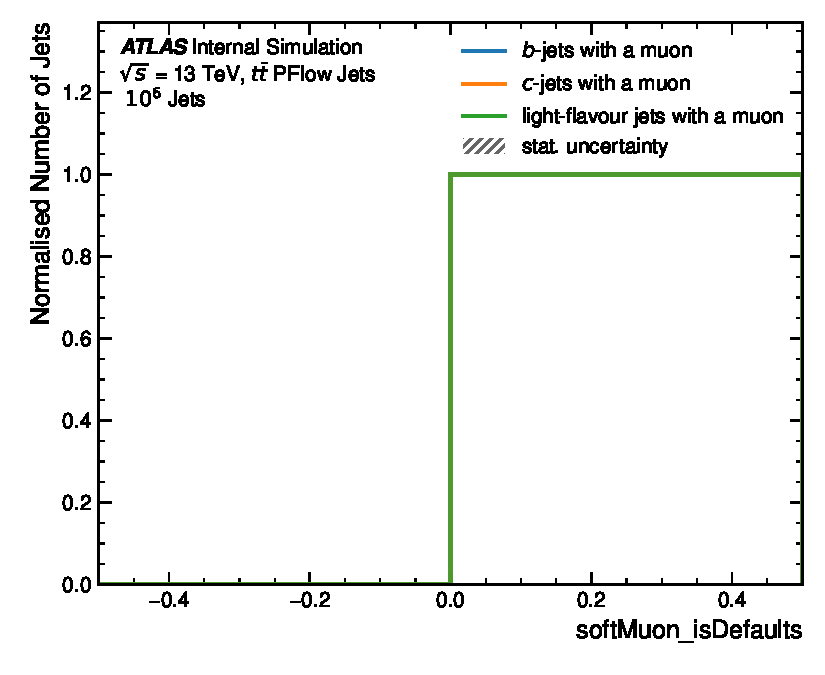
\includegraphics[width=\plotsize\textwidth]{input_vars_smt_ttbar_zpext/softMuon_isDefaults}
    }
    \subfigure[]{
        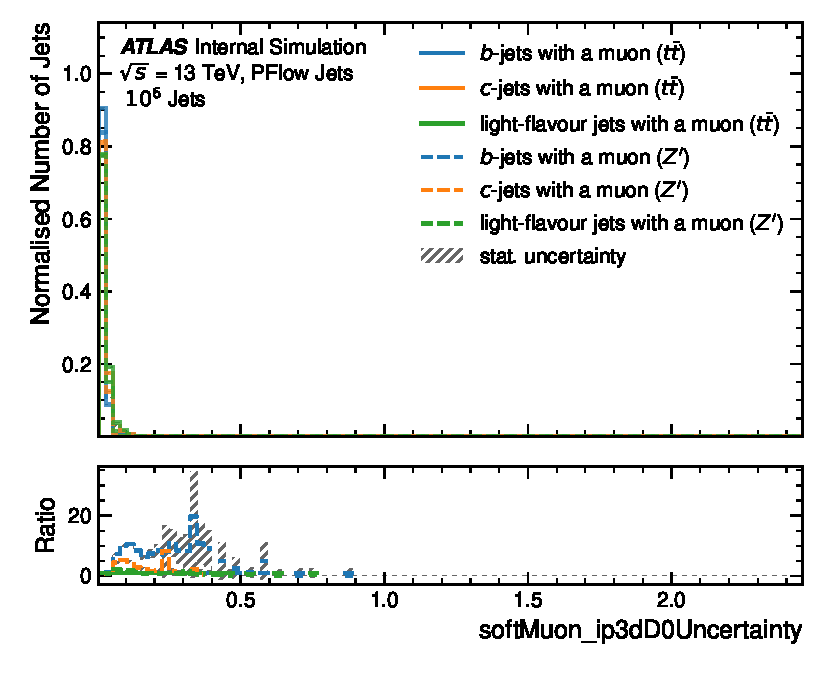
\includegraphics[width=\plotsize\textwidth]{input_vars_smt_ttbar_zpext/softMuon_ip3dD0Uncertainty}
    }
    \subfigure[]{
        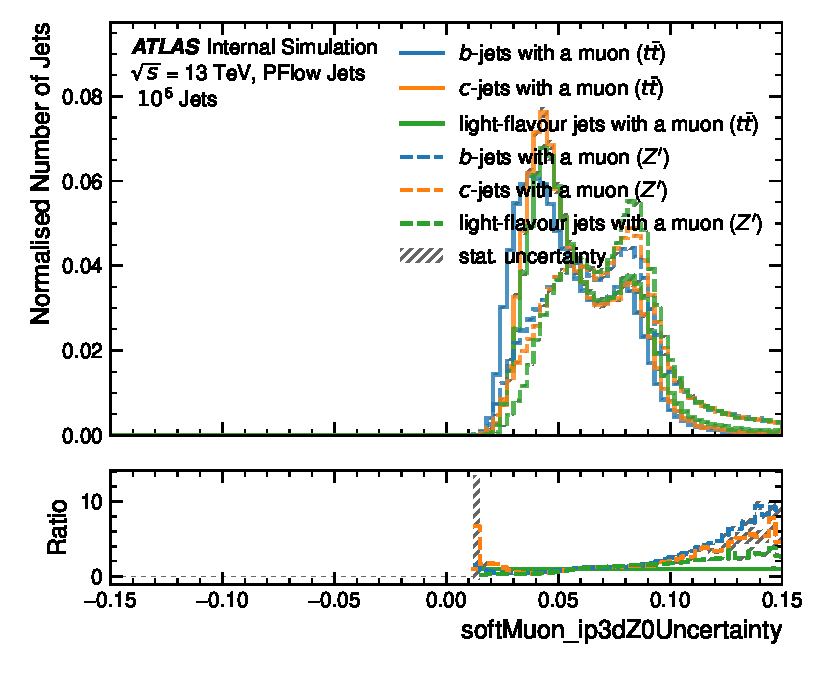
\includegraphics[width=\plotsize\textwidth]{input_vars_smt_ttbar_zpext/softMuon_ip3dZ0Uncertainty}
    }\\
    \subfigure[]{
        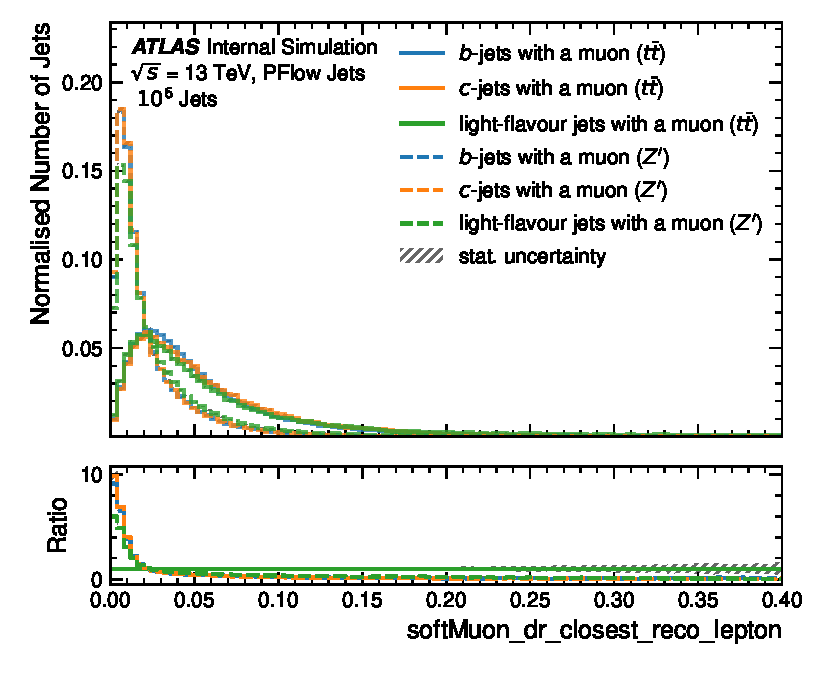
\includegraphics[width=\plotsize\textwidth]{input_vars_smt_ttbar_zpext/softMuon_dr_closest_reco_lepton}
    }
    \subfigure[]{
        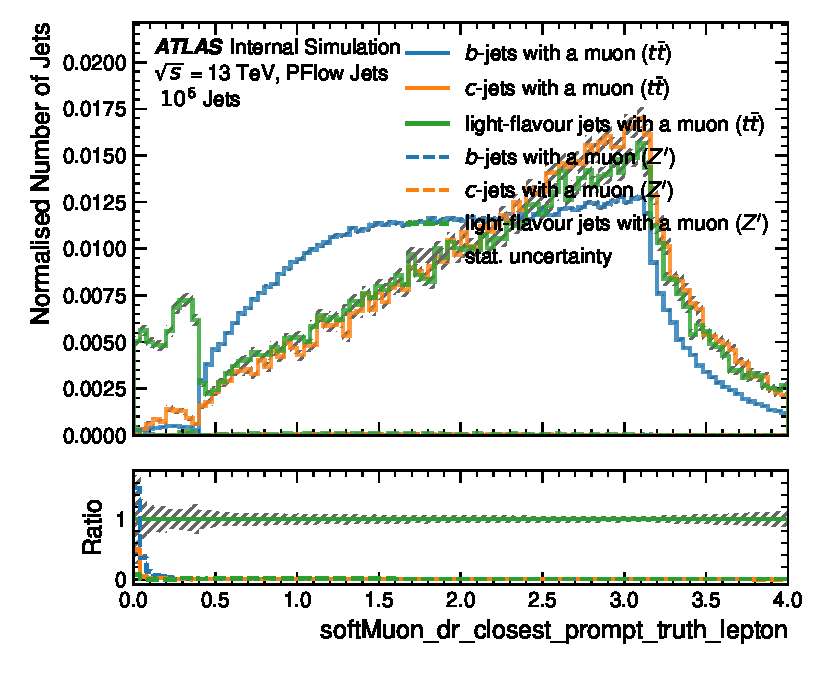
\includegraphics[width=\plotsize\textwidth]{input_vars_smt_ttbar_zpext/softMuon_dr_closest_prompt_truth_lepton}
    }
    \subfigure[]{
        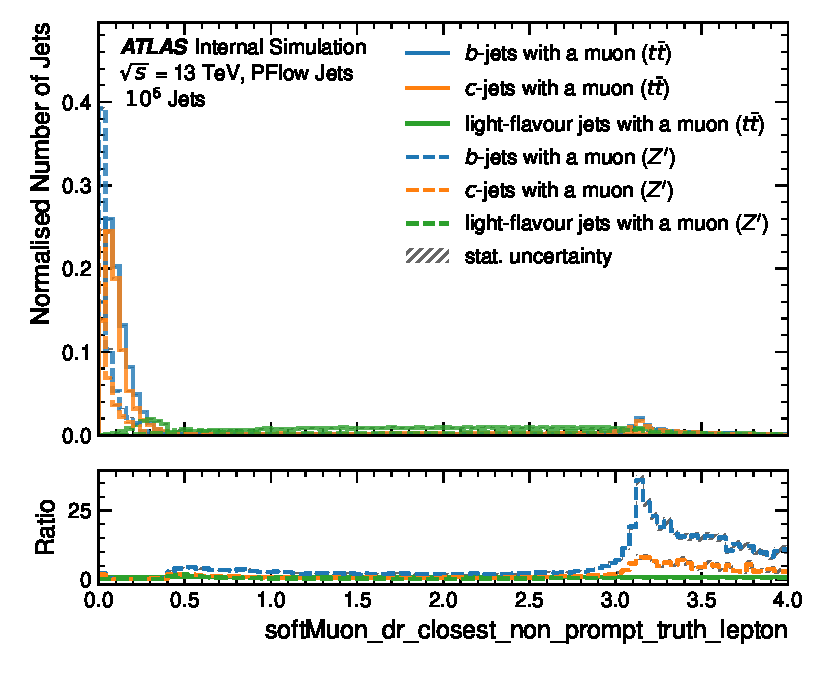
\includegraphics[width=\plotsize\textwidth]{input_vars_smt_ttbar_zpext/softMuon_dr_closest_non_prompt_truth_lepton}
    }\\
    \subfigure[]{
        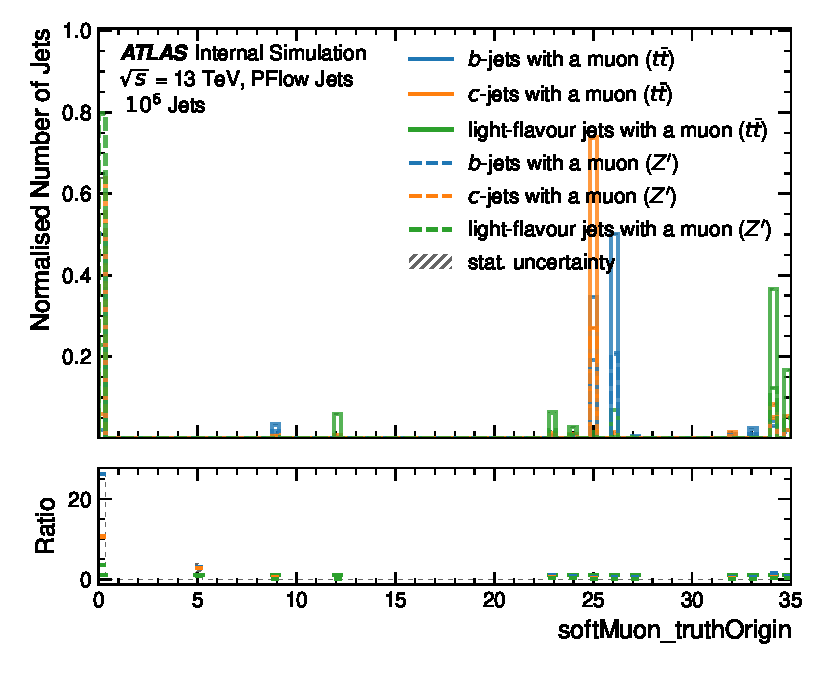
\includegraphics[width=\plotsize\textwidth]{input_vars_smt_ttbar_zpext/softMuon_truthOrigin}
    }
    \subfigure[]{
        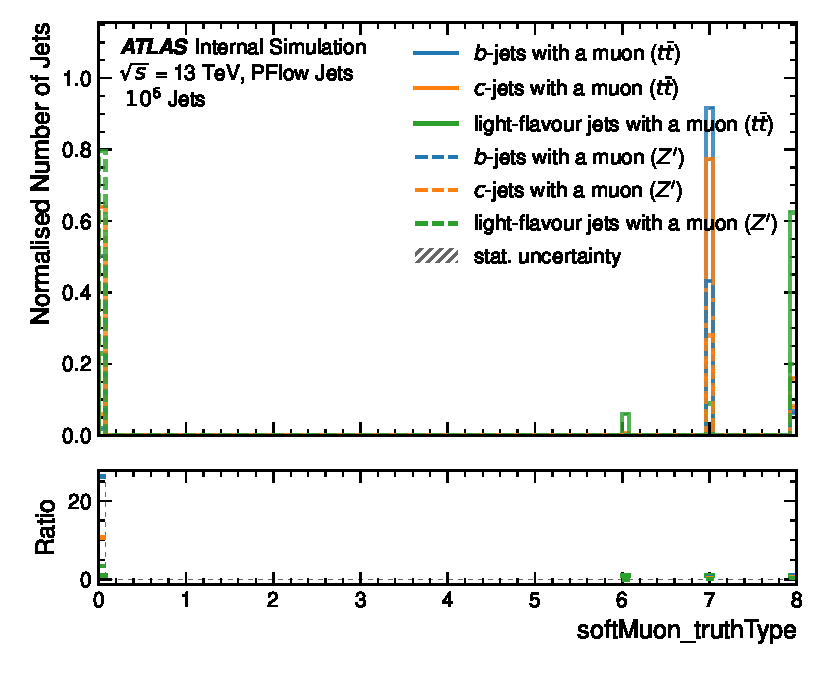
\includegraphics[width=\plotsize\textwidth]{input_vars_smt_ttbar_zpext/softMuon_truthType}
    }
    \subfigure[]{
        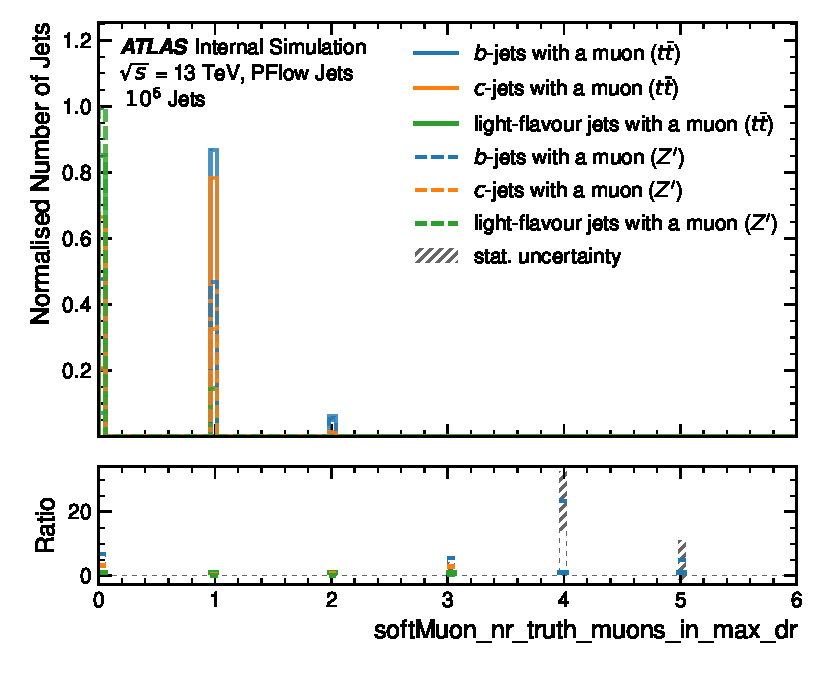
\includegraphics[width=\plotsize\textwidth]{input_vars_smt_ttbar_zpext/softMuon_nr_truth_muons_in_max_dr}
    }\\
    \subfigure[]{
        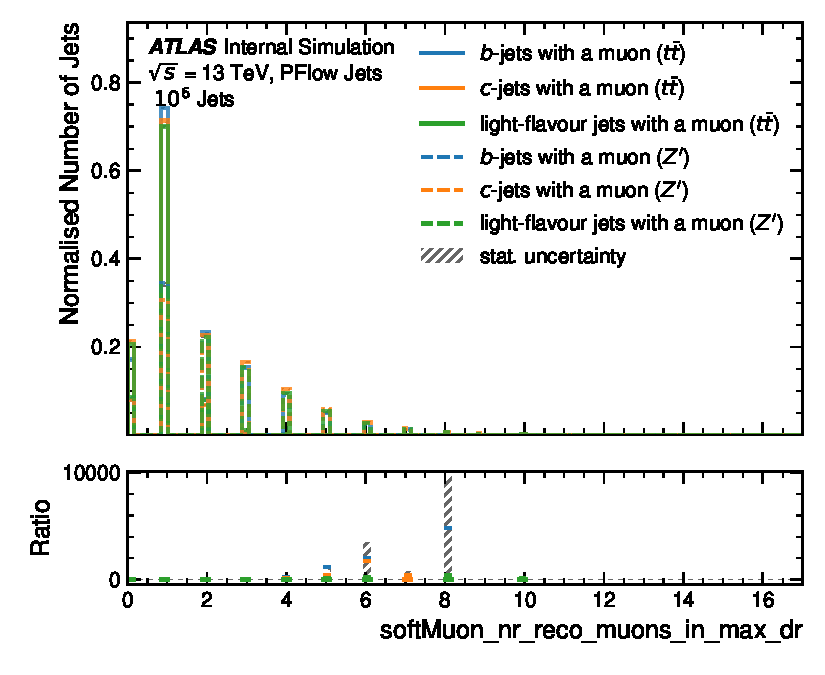
\includegraphics[width=\plotsize\textwidth]{input_vars_smt_ttbar_zpext/softMuon_nr_reco_muons_in_max_dr}
    }
    \subfigure[]{
        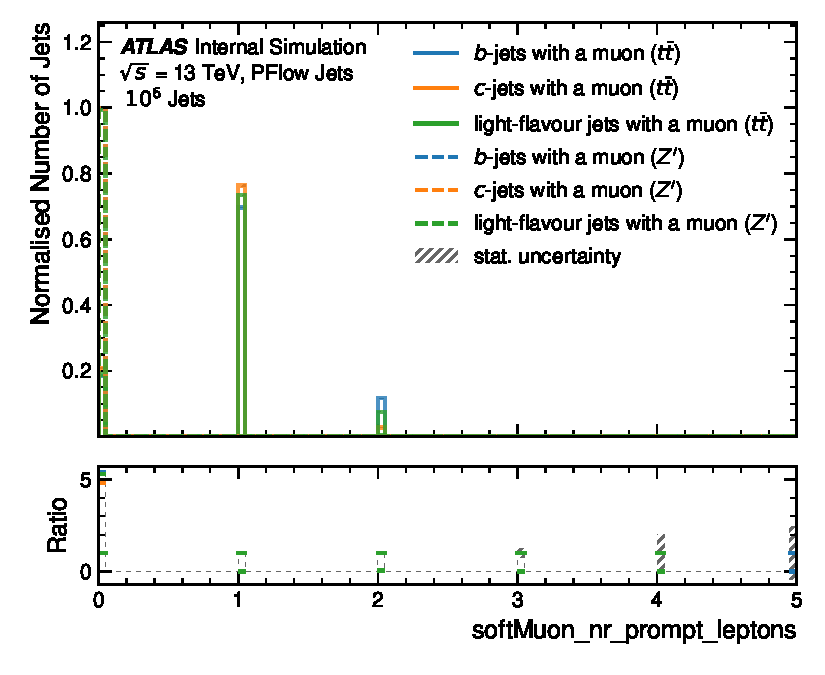
\includegraphics[width=\plotsize\textwidth]{input_vars_smt_ttbar_zpext/softMuon_nr_prompt_leptons}
    }
    \subfigure[]{
        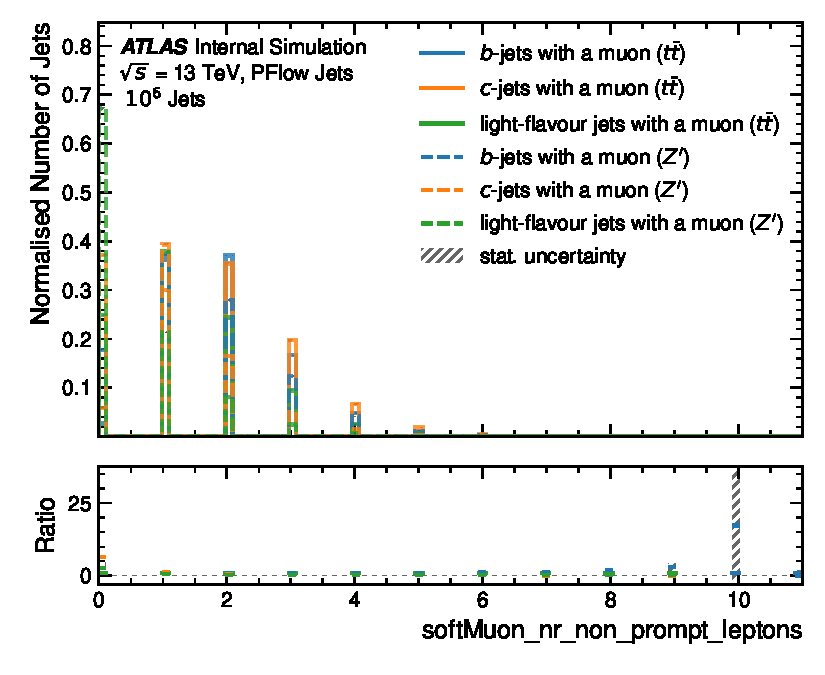
\includegraphics[width=\plotsize\textwidth]{input_vars_smt_ttbar_zpext/softMuon_nr_non_prompt_leptons}
    }
    \caption{Explored muon variables (2/7)}
    \label{fig:smt_vars_2}
\end{figure}







\begin{figure}[]
    \centering
    \subfigure[]{
        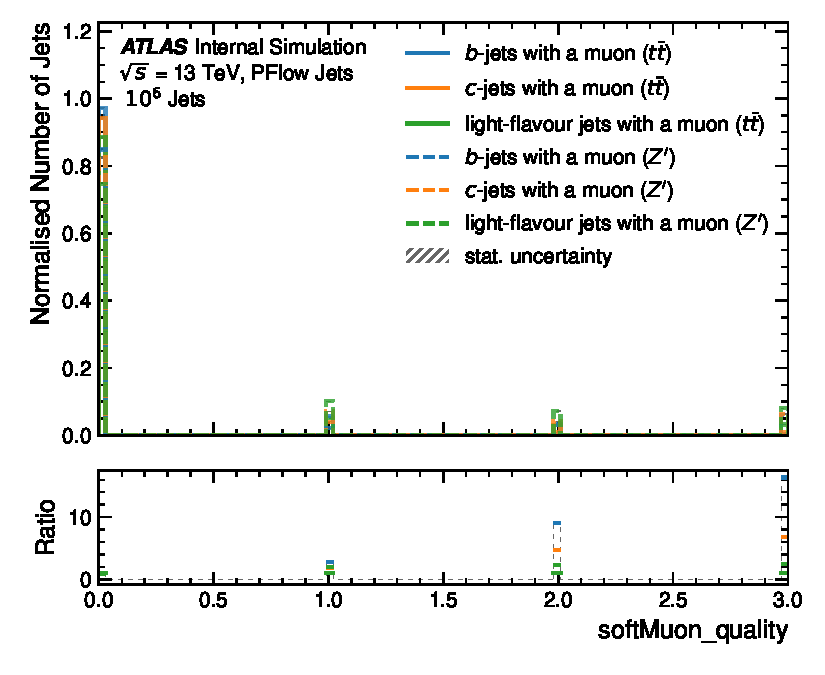
\includegraphics[width=\plotsize\textwidth]{input_vars_smt_ttbar_zpext/softMuon_quality}
    }
    \subfigure[]{
        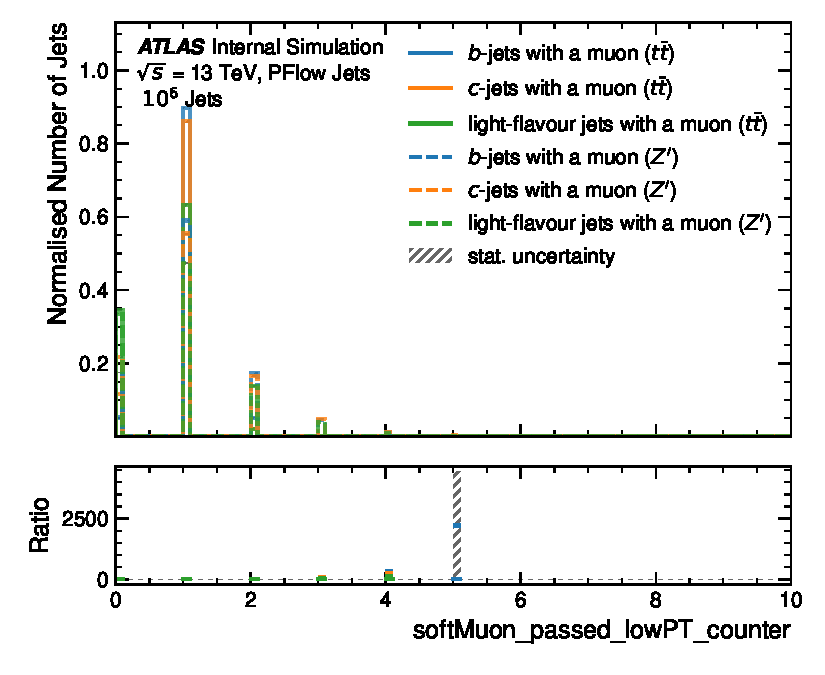
\includegraphics[width=\plotsize\textwidth]{input_vars_smt_ttbar_zpext/softMuon_passed_lowPT_counter}
    }
    \subfigure[]{
        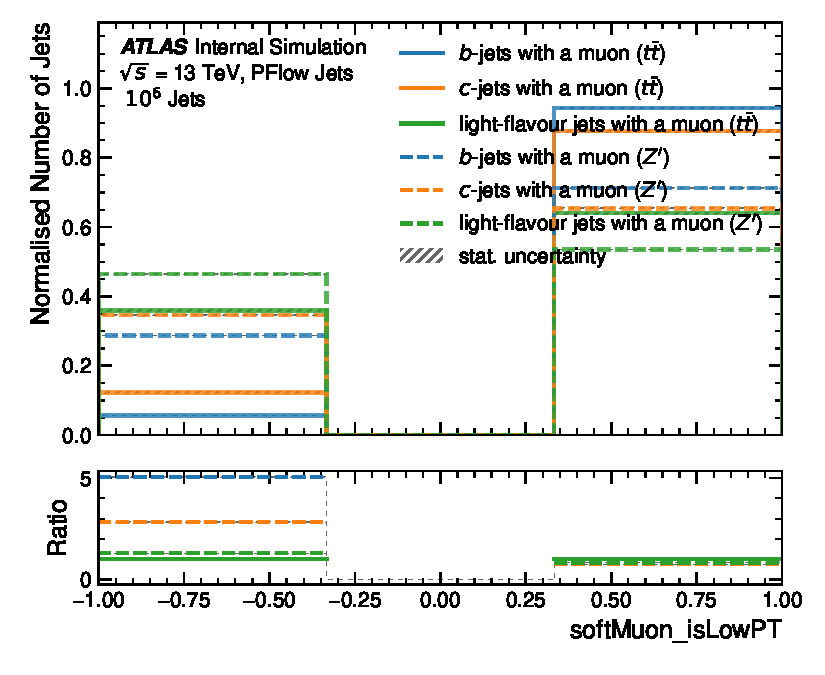
\includegraphics[width=\plotsize\textwidth]{input_vars_smt_ttbar_zpext/softMuon_isLowPT}
    }\\
    \subfigure[]{
        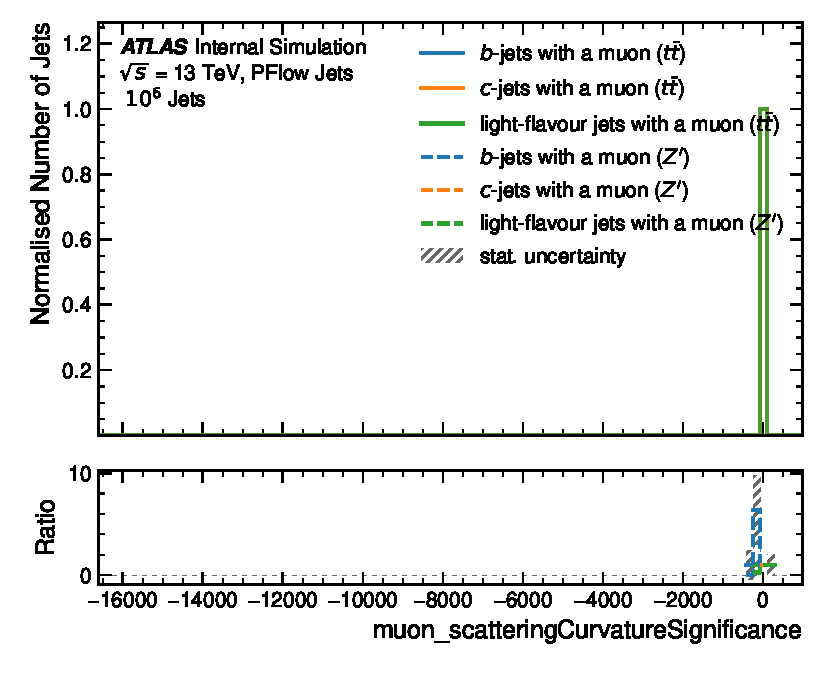
\includegraphics[width=\plotsize\textwidth]{input_vars_smt_ttbar_zpext/muon_scatteringCurvatureSignificance}
    }
    \subfigure[]{
        \includegraphics[width=\plotsize\textwidth]{input_vars_smt_ttbar_zpext/muon_spectrometerFieldIntegral}
    }
    \subfigure[]{
        \includegraphics[width=\plotsize\textwidth]{input_vars_smt_ttbar_zpext/muon_segmentDeltaEta}
    }\\
    \subfigure[]{
        \includegraphics[width=\plotsize\textwidth]{input_vars_smt_ttbar_zpext/muon_segmentDeltaPhi}
    }
    \subfigure[]{
        \includegraphics[width=\plotsize\textwidth]{input_vars_smt_ttbar_zpext/muon_segmentChi2OverDoF}
    }
    \subfigure[]{
        \includegraphics[width=\plotsize\textwidth]{input_vars_smt_ttbar_zpext/muon_t0}
    }\\
    \subfigure[]{
        \includegraphics[width=\plotsize\textwidth]{input_vars_smt_ttbar_zpext/muon_beta}
    }
    \subfigure[]{
        \includegraphics[width=\plotsize\textwidth]{input_vars_smt_ttbar_zpext/muon_annBarrel}
    }
    \subfigure[]{
        \includegraphics[width=\plotsize\textwidth]{input_vars_smt_ttbar_zpext/muon_annEndCap}
    }
    \caption{Explored muon variables (3/7)}
    \label{fig:smt_vars_3}
\end{figure}




\begin{figure}[]
    \centering
    \subfigure[]{
        \includegraphics[width=\plotsize\textwidth]{input_vars_smt_ttbar_zpext/muon_innAngle}
    }
    \subfigure[]{
        \includegraphics[width=\plotsize\textwidth]{input_vars_smt_ttbar_zpext/muon_midAngle}
    }
    \subfigure[]{
        \includegraphics[width=\plotsize\textwidth]{input_vars_smt_ttbar_zpext/muon_msInnerMatchChi2}
    }\\
    \subfigure[]{
        \includegraphics[width=\plotsize\textwidth]{input_vars_smt_ttbar_zpext/muon_msOuterMatchChi2}
    }
    \subfigure[]{
        \includegraphics[width=\plotsize\textwidth]{input_vars_smt_ttbar_zpext/muon_meanDeltaADCCountsMDT}
    }
    \subfigure[]{
        \includegraphics[width=\plotsize\textwidth]{input_vars_smt_ttbar_zpext/muon_CaloLRLikelihood}
    }\\
    \subfigure[]{
        \includegraphics[width=\plotsize\textwidth]{input_vars_smt_ttbar_zpext/muon_FSR_CandidateEnergy}
    }
    \subfigure[]{
        \includegraphics[width=\plotsize\textwidth]{input_vars_smt_ttbar_zpext/muon_EnergyLoss}
    }
    \subfigure[]{
        \includegraphics[width=\plotsize\textwidth]{input_vars_smt_ttbar_zpext/muon_ParamEnergyLoss}
    }\\
    \subfigure[]{
        \includegraphics[width=\plotsize\textwidth]{input_vars_smt_ttbar_zpext/muon_MeasEnergyLoss}
    }
    \subfigure[]{
        \includegraphics[width=\plotsize\textwidth]{input_vars_smt_ttbar_zpext/muon_EnergyLossSigma}
    }
    \subfigure[]{
        \includegraphics[width=\plotsize\textwidth]{input_vars_smt_ttbar_zpext/muon_ParamEnergyLossSigmaPlus}
    }
    \caption{Explored muon variables (4/7)}
    \label{fig:smt_vars_4}
\end{figure}



\begin{figure}[]
    \centering

    \subfigure[]{
        \includegraphics[width=\plotsize\textwidth]{input_vars_smt_ttbar_zpext/muon_ParamEnergyLossSigmaMinus}
    }
    \subfigure[]{
        \includegraphics[width=\plotsize\textwidth]{input_vars_smt_ttbar_zpext/muon_MeasEnergyLossSigma}
    }
    \subfigure[]{
        \includegraphics[width=\plotsize\textwidth]{input_vars_smt_ttbar_zpext/muon_CaloMuonScore}
    }\\
    \subfigure[]{
        \includegraphics[width=\plotsize\textwidth]{input_vars_smt_ttbar_zpext/muon_msInnerMatchDOF}
    }
    \subfigure[]{
        \includegraphics[width=\plotsize\textwidth]{input_vars_smt_ttbar_zpext/muon_msOuterMatchDOF}
    }
    \subfigure[]{
        \includegraphics[width=\plotsize\textwidth]{input_vars_smt_ttbar_zpext/muon_CaloMuonIDTag}
    }\\
    \subfigure[]{
        \includegraphics[width=\plotsize\textwidth]{input_vars_smt_ttbar_zpext/softMuon_numberOfPixelHits}
    }
    \subfigure[]{
        \includegraphics[width=\plotsize\textwidth]{input_vars_smt_ttbar_zpext/softMuon_numberOfPixelSharedHits}
    }
    \subfigure[]{
        \includegraphics[width=\plotsize\textwidth]{input_vars_smt_ttbar_zpext/softMuon_numberOfSCTHits}
    }\\
    \subfigure[]{
        \includegraphics[width=\plotsize\textwidth]{input_vars_smt_ttbar_zpext/softMuon_numberOfSCTSharedHits}
    }
    \subfigure[]{
        \includegraphics[width=\plotsize\textwidth]{input_vars_smt_ttbar_zpext/softMuon_numberOfNextToInnermostPixelLayerHits}
    }
    \subfigure[]{
        \includegraphics[width=\plotsize\textwidth]{input_vars_smt_ttbar_zpext/softMuon_numberOfInnermostPixelLayerHits}
    }
    \caption{Explored muon variables (5/7)}
    \label{fig:smt_vars_5}
\end{figure}


\begin{figure}[]
    \centering

    \subfigure[]{
        \includegraphics[width=\plotsize\textwidth]{input_vars_smt_ttbar_zpext/softMuon_numberOfInnermostPixelLayerSharedHits}
    }
    \subfigure[]{
        \includegraphics[width=\plotsize\textwidth]{input_vars_smt_ttbar_zpext/softMuon_numberOfInnermostPixelLayerSplitHits}
    }
    \subfigure[]{
        \includegraphics[width=\plotsize\textwidth]{input_vars_smt_ttbar_zpext/softMuon_numberOfPixelSplitHits}
    }\\
    \subfigure[]{
        \includegraphics[width=\plotsize\textwidth]{input_vars_smt_ttbar_zpext/softMuon_numberOfUsedHitsdEdx}
    }
    \subfigure[]{
        \includegraphics[width=\plotsize\textwidth]{input_vars_smt_ttbar_zpext/softMuon_numberOfNextToInnermostPixelLayerSharedHits}
    }
    \subfigure[]{
        \includegraphics[width=\plotsize\textwidth]{input_vars_smt_ttbar_zpext/softMuon_numberOfNextToInnermostPixelLayerSplitHits}
    }\\
    \subfigure[]{
        \includegraphics[width=\plotsize\textwidth]{input_vars_smt_ttbar_zpext/softMuon_numberOfPixelSpoiltHits}
    }
    \subfigure[]{
        \includegraphics[width=\plotsize\textwidth]{input_vars_smt_ttbar_zpext/softMuon_numberOfDBMHits}
    }
    \subfigure[]{
        \includegraphics[width=\plotsize\textwidth]{input_vars_smt_ttbar_zpext/softMuon_numberOfSCTSpoiltHits}
    }\\
    \subfigure[]{
        \includegraphics[width=\plotsize\textwidth]{input_vars_smt_ttbar_zpext/softMuon_numberOfTRTHits}
    }
    \subfigure[]{
        \includegraphics[width=\plotsize\textwidth]{input_vars_smt_ttbar_zpext/softMuon_numberOfTRTHighThresholdHits}
    }
    \subfigure[]{
        \includegraphics[width=\plotsize\textwidth]{input_vars_smt_ttbar_zpext/softMuon_numberOfTRTHighThresholdHitsTotal}
    }
    \caption{Explored muon variables (6/7)}
    \label{fig:smt_vars_6}
\end{figure}

\begin{figure}[]
    \centering


    \subfigure[]{
        \includegraphics[width=\plotsize\textwidth]{input_vars_smt_ttbar_zpext/softMuon_numberOfTRTTubeHits}
    }
    \subfigure[]{
        \includegraphics[width=\plotsize\textwidth]{input_vars_smt_ttbar_zpext/softMuon_numberOfTRTXenonHits}
    }
    \subfigure[]{
        \includegraphics[width=\plotsize\textwidth]{input_vars_smt_ttbar_zpext/softMuon_numberOfTRTSharedHits}
    }\\
    \subfigure[]{
        \includegraphics[width=\plotsize\textwidth]{input_vars_smt_ttbar_zpext/softMuon_TRTdEdxUsedHits}
    }
    
    \caption{Explored muon variables (7/7)}
    \label{fig:smt_vars_7}
\end{figure}

\section{Adding a muon quality criterion}
Muons used in the association are as inclusive as possible and therefore apart from the selection mentioned in section \ref{sec:MuonSelection} no further quality criterion are applied initially. In other trainings muons were required to have the  ``low pt'' muon identification working point \citep{ATL-PHYS-PUB-2020-002}. This quality criterion improves the muon selection efficiency for muons in the range particularly relevant for this study $\qty[]{3}{GeV}<\pt < \qty[]{6}{GeV}$ (cf. figure \ref{fig:softMuon_pt}). It reduces the backgrounds by \qty{54}{\percent} for light flavor jets and by \qty{23}{\percent} for tau-jets by keeping \qty{77}{\percent} of the $c$-jets and \qty{90}{\percent} of the $b$-jets (cf. table \ref{tab:lowPtMuonJetFlavors}).
\begin{table}[]
  % \sisetup{group-minimum-digits=4}
  \caption{Fraction of associated low pt working point muons per flavor. Fraction of low pt muons to all associated muons (fractions to table \ref{tab:MuonJetFlavors}), the fraction of muons kept after applying the working point. }%
  \label{tab:lowPtMuonJetFlavors}
  \centering
  \resizebox{0.97\textwidth}{!}{
    \begin{tabular}{%
        l
        c
        c
      }
      \hline
      {Jet flavor} & {Fraction of jets with an associated low pt muon} & Fraction of low pt muons \\
      \hline
      light        & 0.0062                                            & 0.4626                   \\
      c            & 0.0363                                            & 0.7690                   \\
      b            & 0.1338                                            & 0.8979                   \\
      tau          & 0.0096                                            & 0.6956                   \\
      \hline
    \end{tabular}}
\end{table}
One way to introduce this information into the neural network is to add another Boolean input variable \textit{isLowPt} that indicates whether the muon meets the necessary requirements for the identification working point. Another option is to use only the muons that passed the identification working point.

\section{Performance comparison to DL1d}
The various additions of muon information to different trainings of \ac{dl1} is evaluated in figure \ref{fig:DL1dmu_ttbar} and \ref{fig:DL1dmu_zpext}. DL1dmu displays similar to DL1r a \qty{25}{\percent} improvement in the light flavor jet rejection and a \qty{10}{\percent} $c$-flavor jet rejection but does neither improve significantly upon adding the hits variables nor for adding the parameters from the muon combined performance variables. Notably, when the "lowPt" identification working point is applied, DL1dmu shows further improvement in its rejection capabilities. Specifically, there's an additional enhancement of approximately $\sim$\qty{10}{\percent}in rejecting light flavor jets and about $\sim$\SI{5}{\percent} in rejecting $c$-flavor jets.

This is regardless if the more inclusive muons selection is applied only given the boolean \textit{lowPt} information or by using the \textit{lowPt} selected muons only which removes a notable \qty{44}{\percent} of the muons. This means that the neural network does not learn anything from the background muons, and that having a muon associated with a $b$-jet is the strongest indicator for a b-hadron. DL1dmu with the \textit{islowPt} variable improves light flavor rejection by $\sim$\qty{40}{\percent} and c-flavor rejection by $\sim$\qty{30}{\percent} compared to the DL1d training

\begin{figure}[]
  \centering
  \includegraphics[width=1\textwidth]{DL1dmu_ttbar}
  \caption{ROC curves of studied models with reference to a trained DL1d model evaluated on \ttbar.}
  \label{fig:DL1dmu_ttbar}
\end{figure}
\begin{figure}[]
  \centering
  \includegraphics[width=1\textwidth]{DL1dmu_zpext}
  \caption{ROC curves of studied models with reference to a trained DL1d model evaluated on \Zprime.}
  \label{fig:DL1dmu_zpext}
\end{figure}

\section{Feature importance}
To understand the influence of a variable to a training of a neural network it can be evaluated with a framework called \ac{shap} \citep{shap,NIPS2017_7062}. It is based on the idea to turn input features on and off and comparing the \ac{ml} model's prediction for both cases. If this is done for all possible combinations the average importance of a feature for a machine learning model can be estimated with the \ac{shap} value. Large positive or negative \ac{shap} values are thus indicators how significantly a particular input feature influences the model's prediction. In the context of $b$-tagging large negative \ac{shap} values will help the model to better reject whereas features with large positive \ac{shap} values helps the model to learn that these are most probably jets from the output node of interest.

The evaluation for DL1dmu, with the boolean \textit{isLowPt} variable added, is shown in fig. \ref{fig:shapleyDL1dmu}. It clearly shows that main improvements over the previous implementation are due to the addition of the muon \pt and the low pt working point information to DL1dmu.
\begin{figure}[]
  \centering
  \includegraphics[width=1\textwidth]{ttbar_r22_shapley_b-jets}
  \caption{SHAP values for the $b$-jet output node of DL1dmu representing the impact of an input features influence to the neural network.}
  \label{fig:shapleyDL1dmu}
\end{figure}
The evaluation for the model that added all variables is shown in fig. \ref{fig:ttbar_r22_shapley_b_all_vars}. Even though a lot of the \ac{mcp} variables (see table \ref{tab:DL1dModels}) rank mediocre there was basically no improvement in performance (fig. \ref{fig:DL1dmu_ttbar}-\ref{fig:DL1dmu_zpext}).
\begin{figure}[]
  \centering
  \includegraphics[width=0.97\textwidth]{ttbar_r22_shapley_b-jets_all_vars}
  \caption{SHAP values for the $b$-jet output node of the DL1dmu\_all\_vars representing the impact of an input features influence to the neural network.}
  \label{fig:ttbar_r22_shapley_b_all_vars}
\end{figure}
The minimal impact of incorporating most MCP variables on the model's performance is likely due to their strong linear correlation with the muon's transverse momentum \pt. This correlation is clearly evident in the correlation matrix presented in Figure \ref{fig:correlation_matrix}. Since the \pt of the muon is already informatively represented in other variables, such as the Momentum Balance Significance, the additional MCP variables do not contribute significant new information to the model. A more detailed visual representation is shown in scatter plots of Figure \ref{fig:scatterplot_matrix_mcp} showcasing the relationships among \ac{smt} and \ac{mcp} variables.
\begin{figure}[]
  \centering
  \includegraphics[width=1\textwidth]{correlation_matrix}
  \caption{Linear correlations between all explored soft muon variables. E.g. \pt is strongly correlated to ParamEnergyLossSigmaPlus, which in turn is  correlated to ParamEnergyLoss. }
  \label{fig:correlation_matrix}
\end{figure}

\begin{figure}[]
  \centering
  \includegraphics[width=1\textwidth]{scatterplot_matrix_mcp}
  \caption{\ac{smt} and \ac{mcp} variables (see table \ref{tab:smtAbbreviations}) plotted against each other to reveal correlations. Overlays represent one standard deviation scattered points.}
  \label{fig:scatterplot_matrix_mcp}
\end{figure}

% VIVA_13.05.22.pdf ! 

